\documentclass[
	a4paper,
	12pt,
	bibliography=totocnumbered,
	twoside,
	%draft
]{scrreprt}

% ------------------------------------------------------------------------------------------------------------------------ %
%%% Packages & Renews
% ------------------------------------------------------------------------------------------------------------------------ %
\usepackage[ngerman, ngerman]{babel}
\usepackage[T1]{fontenc}
\usepackage[utf8]{inputenc}
\usepackage[a4paper,
						left=2.5cm,
						right=2.5cm,
						top=2.5cm,
						bottom=1.61cm,
						includehead
						]{geometry}

\renewcommand*\chapterheadstartvskip{\vspace*{-\topskip}}
\renewcommand*\chapterheadendvskip{%
  \vspace*{1\baselineskip plus .1\baselineskip minus .167\baselineskip}}
\addtokomafont{sectioning}{\rmfamily}


% ----- Mathematische Symbole ----- %
\usepackage{amssymb,amsmath}
\DeclareMathOperator*{\argmin}{arg\,min}												% argmin-Operator


% ----- Schriftart ----- %
\usepackage{mathptmx}					% Times New Roman als Schrift


% ----- Text -----%
\usepackage{soul}							% strikethrough text with \st{text}

% ----- Farben ----- %
\usepackage{color}						% Schriftfarbe, wechseln z.Bsp. via \color{red}
%\usepackage[usenames, dvipsnames}{xcolor}
\usepackage{colortbl}					% Farben in Tabellen


\definecolor{tubs_red}{rgb}{0.75, 0.12, 0.24}

\definecolor{codegreen}{rgb}{0,0.6,0}
\definecolor{codegray}{rgb}{0.5,0.5,0.5}
\definecolor{codepurple}{rgb}{0.58,0,0.82}
\definecolor{codeblue}{rgb}{0,0.05,0.72}
\definecolor{codeblack}{rgb}{0,0,0}

% TU BS Sekundärfarbe blau
\definecolor{tubs_blue_light}{rgb}{0.4, 0.71, 0.83}													% hellblau
\definecolor{tubs_blue_light80}{rgb}{0.52, 0.76, 0.86}											% hellblau 80%
\definecolor{tubs_blue_light60}{rgb}{0.64, 0.82, 0.90}											% hellblau 60%
\definecolor{tubs_blue_light40}{rgb}{0.76, 0.88, 0.93}											% hellblau 40%
\definecolor{tubs_blue_light20}{rgb}{0.88, 0.94, 0.96}											% hellblau 20%

\definecolor{tubs_blue}{rgb}{0.00, 0.44, 0.61}															% blau
\definecolor{tubs_blue80}{rgb}{0.20, 0.55, 0.69}														% blau 80%
\definecolor{tubs_blue60}{rgb}{0.40, 0.66, 0.76}														% blau 60%
\definecolor{tubs_blue40}{rgb}{0.60, 0.78, 0.84}														% blau 40%
\definecolor{tubs_blue20}{rgb}{0.80, 0.87, 0.92}														% blau 20%

\definecolor{tubs_blue_dark}{rgb}{0.00, 0.25, 0.34}													% dunkelblau
\definecolor{tubs_blue_dark80}{rgb}{0.20, 0.40, 0.47}												% dunkelblau 80%
\definecolor{tubs_blue_dark60}{rgb}{0.40, 0.55, 0.60}												% dunkelblau 60%
\definecolor{tubs_blue_dark40}{rgb}{0.60, 0.70, 0.74}												% dunkelblau 40%
\definecolor{tubs_blue_dark20}{rgb}{0.80, 0.85, 0.87}												% dunkelblau 20%



\usepackage{eurosym}				% Euro-Symbol via \EUR{ } oder \euro
%\usepackage{longtable}			%Tabellen über mehr als eine Seite
\usepackage{array}            %mehr Befehe für Tabellen
\usepackage{stmaryrd}	%Widerspruchsblitz
\usepackage[bottom]{footmisc} % Fußnoten unter Abb.


% ----- Abkürzungen ----- %
\usepackage{acronym}



% ----- Verweise im Text ----- %
\usepackage{hyperref}


% ----- Listings für Code ----- %
\usepackage{listings}

\lstdefinestyle{mystyle}{
    backgroundcolor=\color{white},   
    commentstyle=\color{codegreen},
    keywordstyle=\color{codeblue},
    numberstyle=\tiny\color{codegray},
    stringstyle=\color{codepurple},
    basicstyle=\ttfamily\scriptsize,                							% ttfamily = Monospace, scriptsize = 12pt->8pt
    breakatwhitespace=true,                         							% allow line break only at whitespace
    breaklines=true,
    captionpos=b,
    keepspaces=true,
    numbers=left,
    stepnumber=1,                                   							% number on every n-th line
    emptylines=2,                                   							% Max. 2 empty lines in code
    extendedchars=true,
    numbersep=10pt,
    showspaces=false,                               							% do not show spaces
    showstringspaces=false,
    showtabs=false,
    tabsize=2,
    frame=single,                                  		 						% frame around cond
    rulecolor=\color{codeblack}
}
 % Anwenden
\lstset{style=mystyle}
\renewcommand{\lstlistingname}{Quellcode}           							% change caption to "quellcode"
\renewcommand{\lstlistlistingname}{Quellcodeverzeichnis}       		% "list of listing" -> "Quellcode-Verzeichnis"




% ----- Fußnoten ----- %
\usepackage{tablefootnote}																				% to use footnotes inside mdtheorems	




% ----- Abbildungen ----- %
\usepackage{graphicx}															% Einbinden von Bildern
\usepackage{calc}																	% Berechnen von Längen, z. B. bei 0.5\textwidth
\usepackage{float}																% Abb.& Tabellen exakt einbinden mit [H]-Zusatz
\usepackage[labelfont=bf]{caption}								% 'Abbildung X' fett
\counterwithout{figure}{chapter}									% Abbildungen fortlaufend nummerieren, ohne Kapitelangabe




% ----- Kopf- und Fußzeile einrichten ----- %
\usepackage[headsepline]{scrpage2}
\pagestyle{scrheadings}
\clearscrheadfoot
\ohead{\pagemark} 																% Kopfzeile außen:  Seitenzahl
\ihead{\headmark}																	% Kopfzeile innen:  Kapitel / Abschnitt

%\setkomafont{pagefoot}{
%\normalfont\sffamily}
\automark[section]{chapter}

% ----- Zeilenabstand einstellen ----- %
\linespread{1.43}		 															% Zeilenabstand 1.5fach




\setlength{\parindent}{0cm}

% ----- Sätze, Theoreme, Beispiele, Definitionen ----- %
%\theoremstyle{definition}
%\newtheorem{Definition}{Definition}[chapter]
%\newtheorem{Korollar}{Korollar}[chapter]
%\newtheorem{Satz}{Satz}[chapter] % Umgebungsname=Satz, sichtbarer Name = Satz, Zähler = chapterweise neu beginnen
%\newtheorem{Bsp}[Satz]{Beispiel}

% ----- Definitionen, Sätze, ... ----- %
\usepackage{mdframed}
% Definition
\mdtheorem[
	linecolor=tubs_blue_light,
	frametitlefont=\bfseries\color{black},
	frametitlebackgroundcolor=tubs_blue_light60,
  frametitlerule=true,
	frametitleaboveskip=2pt,
	frametitlebelowskip=2pt,
	footnoteinside=false,
	]{Definition}{Definition}[chapter]
	
% Beispiel
\mdtheorem[
	linecolor=tubs_blue_light,
	frametitlefont=\bfseries\color{black},
	frametitlebackgroundcolor=tubs_blue_light60,
  frametitlerule=true,
	frametitleaboveskip=2pt,
	frametitlebelowskip=2pt,
	footnoteinside=false,
	]{Beispiel}{Beispiel}[chapter]

% Satz
\mdtheorem[
	linecolor=tubs_blue,
	frametitlefont=\bfseries\color{black},
	frametitlebackgroundcolor=tubs_blue60,
  frametitlerule=true,
	frametitleaboveskip=2pt,
	frametitlebelowskip=2pt,
	footnoteinside=false,
	]{Satz}{Satz}[chapter]

% Korollar
\mdtheorem[
	linecolor=tubs_blue,
	frametitlefont=\bfseries\color{black},
	frametitlebackgroundcolor=tubs_blue60,
  frametitlerule=true,
	frametitleaboveskip=2pt,
	frametitlebelowskip=2pt,
	footnoteinside=false,
	]{Korollar}{Korollar}[chapter]



%
%
%
%
\newcommand{\qed}{\qquad \hfill \fbox{}\\}		%Beweiskasten, danach neue Zeile

%Einbindung einer pdf-Datei
\usepackage{pdfpages}


% ----- Fußnoten ----- %
\usepackage{chngcntr}
\counterwithout{footnote}{chapter} 																			% fortlaufend nummerieren
\deffootnote[1em]{1em}{1.5em}{\textsuperscript{\thefootnotemark}} 			% 2. Zeile einrücken
\setlength{\footnotesep}{1em} 																					% line height in footnotes


% ----- Abbildungen ----- %
\usepackage[format=plain]{caption}
\captionsetup[figure]{font=footnotesize,
											labelfont=bf											
											}


\usepackage{afterpage}
\renewcommand{\tablename}{\normalsize Table:}

\captionsetup[lstlisting]{font=footnotesize,											% Anpassen der Schriftgröße für captions
											labelfont=bf}
\captionsetup[table]{font=footnotesize,											% Anpassen der Schriftgröße für captions
											labelfont=bf}
											

% ----- Literaturverzeichnis ----- %
\usepackage[babel,
						german=quotes
					 ]{csquotes}
\usepackage[backend=biber,
						style=authoryear,
						natbib
					 ]{biblatex}
\ExecuteBibliographyOptions{
	sorting = nyt, 																% Sort: Autor, Titel, Jahr
	bibwarn = true, 															% Warnings anzeigen
	isbn = false,																	% keine ISBN anzeigen
	url = false, 																	% keine URLs anzeigen
	doi = false		  															% keine DOIs anzeigen
}
\addbibresource{datenbank.bib}



% ------------------------------------------------------------------------------------------------------------------------ %
%%% BEGIN
% ------------------------------------------------------------------------------------------------------------------------ %
\begin{document}


\pagenumbering{gobble}

% ----- Inhaltsverzeichnis ------ %
\setcounter{tocdepth}{1} 
\setcounter{secnumdepth}{4}




% ------------------------------------------------------------------------------------------------------------------------ %
%%% Titelseite
% ------------------------------------------------------------------------------------------------------------------------ %

\begin{figure}[h]
	\vspace{-1.25cm}
	\hspace{-1cm}
	\includegraphics[scale=1.0]{images/tubs_logo.eps}
	\hspace{7.5cm}
	
\includegraphics[scale=0.7]{images/fiwi_logo.eps}
\end{figure}

\hspace{5cm}

\begin{center}

	\vspace{3cm}

	\begin{huge}
		\textbf{Auswirkungen von Meldungen in sozialen Medien auf Aktienmärkte}\\
	\end{huge}
	
	\vspace{0.5cm}
	
	\begin{large}
		Impact of social media announcements on stock markets
	\end{large}
	
	\vspace{1.5cm}
	
	\begin{LARGE}
		\textbf{Bachelorarbeit}
	\end{LARGE}
	
\end{center}

\vspace{\fill}


% Persönliche Informationen
\begin{tabular}{ll}
	\multicolumn{2}{l}{Vorgelegt von:} \\
	\multicolumn{2}{l}{\textbf{Andreas Credé}} \\
	\multicolumn{2}{l}{Jahnallee 2} \\
	\multicolumn{2}{l}{04109 Leipzig} \\
	\ & \ \\
	\textbf{Matrikelnummer:} & 4704513 \\
	\textbf{Studiengang:} & Finanz- und Wirtschaftsmathematik \\
	\ & \ \\
	\textbf{Prüfer:} & Prof. Dr. Marc Gürtler \\
	\textbf{Abgabetermin:} & 05.03.2020 \\
\end{tabular}



%\vspace{\fill}

\thispagestyle{empty}



\pagenumbering{Roman}




% ------------------------------------------------------------------------------------------------------------------------ %
%%% Die super wichtige leere Seite
% ------------------------------------------------------------------------------------------------------------------------ %
\newpage
\null
\thispagestyle{empty}
\newpage



% ------------------------------------------------------------------------------------------------------------------------ %
%%% Eigenständigkeitserklärung
% ------------------------------------------------------------------------------------------------------------------------ %
\addcontentsline{toc}{chapter}{Aufgabenstellung}
\includepdf{images/Aufgabenstellung.pdf}


% ------------------------------------------------------------------------------------------------------------------------ %
%%% Eigenständigkeitserklärung
% ------------------------------------------------------------------------------------------------------------------------ %
\addcontentsline{toc}{chapter}{Erklärung der Eigenständigkeit}

\vspace{6cm}

Hiermit versichere ich, dass ich die vorliegende Arbeit selbständig verfasst und keine anderen als die genehmigten oder angegebenen Quellen und Hilfsmittel benutzt habe.\\

Ferner versichere ich, dass es sich hier um eine Originalarbeit handelt, die noch nicht in einer anderen Prüfung vorgelegen hat.
\vspace{2cm}

\line(1,0){200}	
\newline
Braunschweig, 4. März 2020\\

	

\clearpage
\newpage
\newpage


% ------------------------------------------------------------------------------------------------------------------------ %
%%% Inhaltsverzeichnis
% ------------------------------------------------------------------------------------------------------------------------ %
\tableofcontents
\clearpage



% ------------------------------------------------------------------------------------------------------------------------ %
%%% Abkürzungsverzeichnis
% ------------------------------------------------------------------------------------------------------------------------ %
\chapter*{Abkürzungsverzeichnis}
\addcontentsline{toc}{chapter}{Abkürzungsverzeichnis}

\begin{acronym}[Blash]
	\acro{ADF}{Augmented Dickey-Fuller Test}
	\acro{AIC}{Akaike-Informationskriterium (\textit{Akaike information criterion})}
	\acro{API}{Application Programming Interface}
	\acro{AR}{Autoregression}
	\acro{HTTP}{Hypertext Transfer Protocol}
	\acro{JSON}{JavaScript Object Notation}
	\acro{MAPE}{Mean average percentage error}
	\acro{MSE}{mean squared error}
	\acro{NLP}{Natural Language Processing}
	\acro{NLTK}{Natural Language Toolkit}
	\acro{OAuth}{Open Authorization}
	\acro{POS}{Part-of-speech}
	\acro{REST}{Representational State Transfer}
	\acro{RMSE}{Root-mean-square error}
	\acro{SQL}{Structured Query Language}
	\acro{STTS}{Stuttgart-Tübingen Tagset}
	\acro{VADER}{Valence Aware Dictionary and Sentiment Reasoner}
	\acro{VAR}{Vektorautoregression}
\end{acronym}



% ------------------------------------------------------------------------------------------------------------------------ %
%%% Abbildungsverzeichnis
% ------------------------------------------------------------------------------------------------------------------------ %
\addcontentsline{toc}{chapter}{\listfigurename}
\setcounter{tocdepth}{1}
\listoffigures



% ------------------------------------------------------------------------------------------------------------------------ %
%%% Tabellenverzeichnis
% ------------------------------------------------------------------------------------------------------------------------ %
\addcontentsline{toc}{chapter}{Tabellenverzeichnis}
\listoftables




% ------------------------------------------------------------------------------------------------------------------------ %
%%% 1. Einleitung
% ------------------------------------------------------------------------------------------------------------------------ %
\newpage
\pagenumbering{arabic}
\chapter{Einleitung}
Über den Einfluss der sozialen Medien auf unseren Alltag wird sehr oft spekuliert. Facebook, YouTube und Instagram beeinflussen schon lange unser Konsumverhalten, sowohl durch zielgerichtete Werbung als auch durch unterbewusste Beeinflussung. Die Vermutung liegt nahe, dass auch andere Teile unseres alltäglichen Lebens von den sozialen Medien beeinflusst werden. Bereits 2013 zeigte eine Umfrage unter 360 britischen Finanzexperten\footnote{Vgl. \citet{colt2013}.}, dass deren Mehrheit an den Einfluss der Inhalte sozialer Medien auf die Bewertung von Aktien glaubte. Trotz des Konsenses verwendeten damals nur 7\% der befragten Finanzexperten diese Erkenntnis selbst in ihren Analysen als Indikator. Die Dissonanz zwischen dem empfundenem Einfluss der sozialen Medien auf den Aktienmarkt und der tatsächlichen Untersuchung durch die Erforschung dieses Gebietes zeigt einen sehr großen Handlungsbedarf auf, weswegen die folgende Arbeit sich mit dem Einfluss der sozialen Medien auf die Aktienkurse beschäftigen wird.\\

Die technische Analyse\footnote{Mit der technischen Analyse wird ein Form der Finanzanalyse bezeichnet, die sich allein auf die Kurs- und Umsatzhistorie eines Wertes bezieht.} verwendet bereits seit Jahren Indikatoren, um die Stimmung an den Märkten abzubilden und daraus Handelsentscheidungen abzuleiten. So lässt sich zum Beispiel aus der Put-Call-Ratio, d.h. dem Verhältnis von gehandelten Verkaufs- zu Kaufoptionen, der Verkaufsdruck in einem Markt direkt aus den Umsatzzahlen ermitteln\footnote{Vgl. \citet{murphy2014}, S. 186.}. Andere Indikatoren werden aufgrund von Umfragen unter Marktteilnehmern ermittelt. So erfragt beispielsweise die \textit{American Association of Individual Investors} wöchentlich unter Privatanlegern die erwartete Entwicklung der Aktienmärkte in den nächsten sechs Monaten. Eine ähnliche Umfrage unter Anlageberatern wird seit 1963 regelmäßig vom US-amerikanischen Forschungsinstitut \textit{Investors Intelligence} durchgeführt.
Bei all diesen Indikatoren werden jedoch nur Meinungen spezieller Gruppen von Marktteilnehmern analysiert -- einen (öffentlich zugänglichen) Indikator für eine "`allgemeine"' Stimmung gibt es nicht, obwohl die Daten in Form von Facebook-Statusmeldungen, Instagram-Posts und Tweets etc. öffentlich zugänglich sind. Das folgende Beispiel zeigt, wie stark selbst der Einfluss einzelner Tweets auf den Aktienkurs eines Unternehmens sein kann.\\


\begin{Beispiel}[Einführendes Beispiel]
	\label{bsp:introduction}

	\begin{figure}[H]
		\centering
		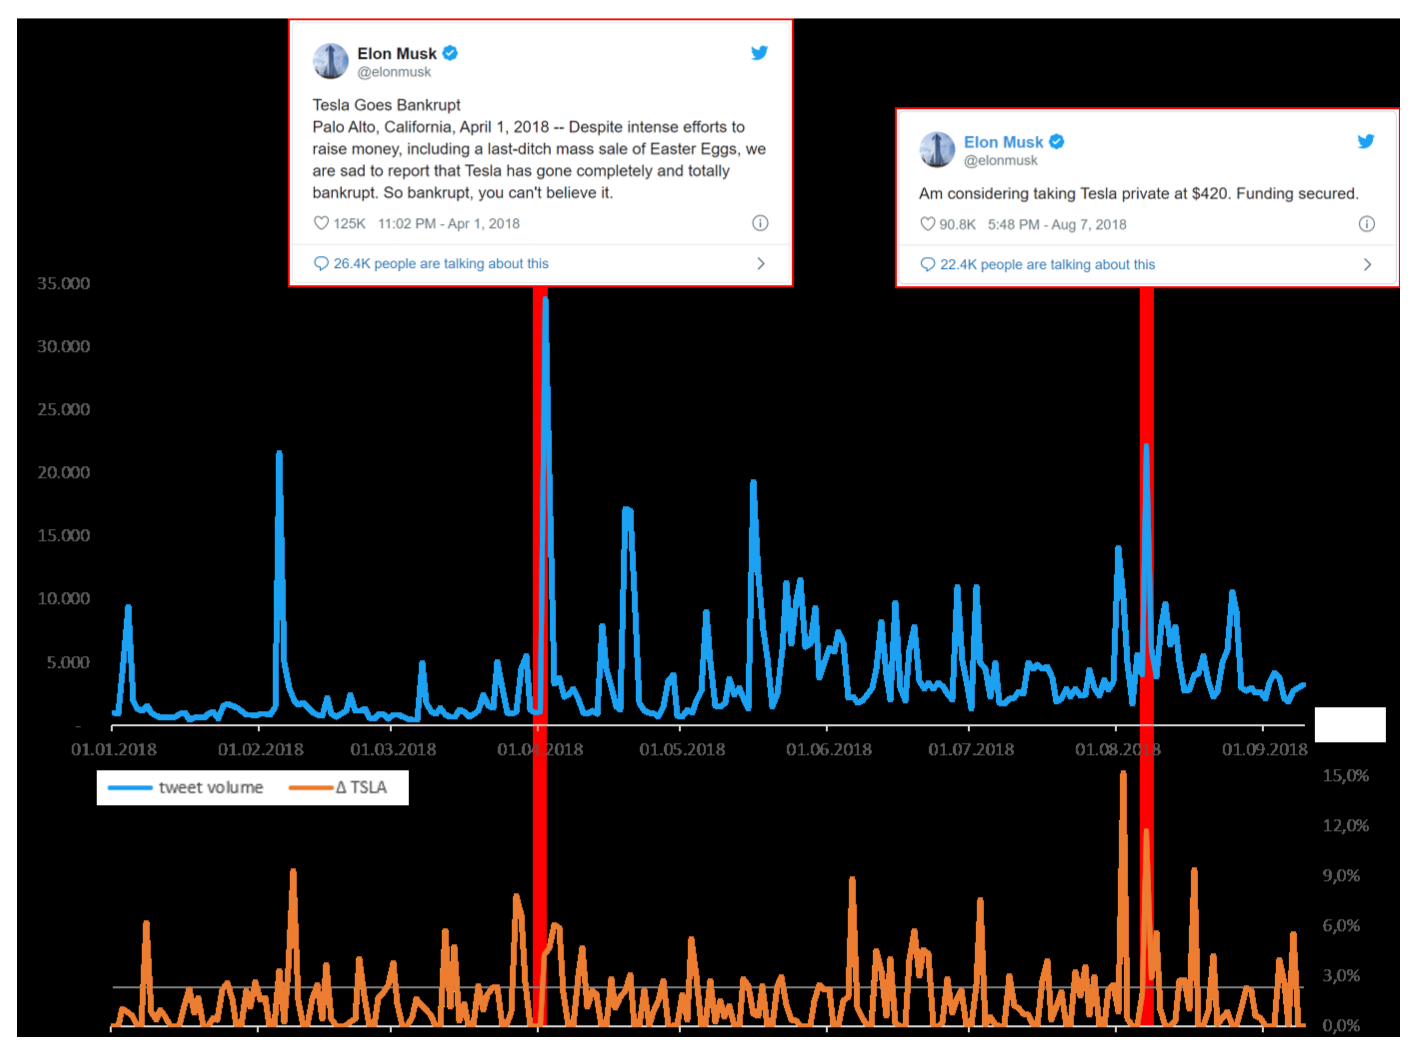
\includegraphics[width=\textwidth]{images/intro_example_tesla_2018_conversation_volume_vs_stock.eps}
		\caption[Tweet-Volumen über Tesla]{Anzahl Tweets pro Tag (hellblau) über Tesla und dessen Vorstandsvorsitzenden, Elon Musk (01.2018 - 09.2018), Aktienkurs von Tesla (orange), Mittlere absolute Veränderung des Kurses (grau)}
		\label{img:tesla-2018}
	\end{figure}

	Abbildung \ref{img:tesla-2018} zeigt das Aufkommen an Tweets über Tesla (unter dem Hashtag \#tesla) und über den Gründer und Vorstandsvorsitzenden Elon Musk (Twitter-Nutzer @elonmusk). Deutlich erkennbar sind die beiden Spitzen in der Anzahl der Tweets im April und August, die in Zusammenhang mit den kontrovers diskutierten Tweets von Elon Musk stehen. Abbildung \ref{img:tesla-2018} zeigt in der unteren Zeitreihe die Schwankungen\footnotemark in Teslas Aktienkurs im selben Zeitraum und die deutlich erkennbare höhere Schwankung (4,26\% bzw. 11,72\% vs. durchschnittlichen 2,33\% täglicher Schwankung) des Aktienkurses an Tagen mit kontroversen Tweets über das Unternehmen.\\

	Ausschläge wie dieser legen nahe, dass es einen Zusammenhang zwischen der Stimmung in sozialen Netzwerken und dem Aktienkurs eines Unternehmens geben könnte. Sie zeigen aber auch, dass der Inhalt der Nachrichten über die Richtung des Kurses entscheidend sein kann. So gab der Aktienkurs nach dem "`Aprilscherz-Tweet"' vom 1. April 2018 nach, während er nach dem "Privatisierungs-Tweet" vom 7. August 2018 deutlich zunahm.
\end{Beispiel}
\footnotetext{Gemessen wurde die Veränderung zum Vortag in Prozent.}
\bigskip
Die folgende Arbeit gliedert sich in drei Teile. Im ersten Teil wird zunächst ein Überblick über bisherige Forschungsarbeiten mit ähnlichen Fragestellungen gegeben. Dabei werden die verwendeten Modelle vorgestellt und hinsichtlich ihrer Prognosegüte verglichen. Der zweite Teil behandelt die Erfassung und Verarbeitung von Texten, die zur Entwicklung einer Stimmungsvariablen notwendig sind. Dabei werden zunächst die Grundlagen der Computerlinguistik erklärt und ein Modell zur lexikonbasierten Sentiment-Analyse von Texten vorgestellt. Anschließend wird der im Rahmen dieser Arbeit erhobene Textkorpus\footnote{Als Textkorpus wird eine Sammlung schriftlicher Texte bezeichnet, die meist einer gemeinsamen Sprache oder Textgattung angehören.} mit den vorgestellten Methoden analysiert und daraus eine Variable für die Stimmung abgeleitet. Im dritten Teil wird eine Einführung in vektorautoregressive Modelle für Zeitreihen gegeben und wie sich daraus Prognosen erzeugen lassen. Auf Basis der in Teil 2 entwickelten Variable wird schließlich ein Modell trainiert und die Güte der daraus erzeugten Prognose analysiert.




% ------------------------------------------------------------------------------------------------------------------------ %
%%% Hauptteil
% ------------------------------------------------------------------------------------------------------------------------ %


% ------------------------------------------------------------------------------------------------------------------------ %
%%% Kapitel 2: Verwandte Arbeiten
% ------------------------------------------------------------------------------------------------------------------------ %
\chapter{Verwandte Arbeiten}
\label{ch:similiar-work}

In diesem Kapitel werden verwandte Arbeiten mit ähnlichen Fragestellungen vorgestellt und hinsichtlich ihrer verwendeten Methoden und der Güte der verwendeten Modelle analysiert und verglichen.\\


%%% 2.1: Überblick --------------------------------------------------------------------------------------------------------%
\section{Überblick}
Zahlreiche Arbeiten wurden bereits dem Thema der Prognose von Aktienkursen gewidmet. Frühe Forschungsansätze gehen dabei oft von der Annahme der Markteffizienzhypothese\footnote{Vgl. \citet{fama1965}.} und der Random-Walk-Theorie\footnote{Vgl. \citet{fama1969}.} aus, nach denen Aktienkurse nur von neuen Informationen beeinflusst werden und sich nicht aufgrund von Vergangenheitswerten vorhersagen lassen. Demzufolge dürfte kein Marktteilnehmer in der Lage sein, überdurchschnittliche Gewinne zu erwirtschaften und eine Vorhersage eines Aktienkurses dürfte eine Genauigkeit von 50\% langfristig nicht überschreiten.\\

Obwohl Eugene Fama 2013 für seine Forschungen auf diesem Gebiet der Alf\-red-Nobel-Ge\-dächt\-nis\-preis für Wirtschaftswissenschaften verliehen wurde, konnte in jüngeren Forschungen die Annahme widerlegt werden, dass Aktienkurse einem Random-Walk folgen\footnote{Vgl. \citet{qian2007}.}. Andere Untersuchungen versuchten die These zu widerlegen, dass Ereignisse und die daraus resultierenden Nachrichten re	in zufällig und damit unvorhersehbar sind. Die zunehmende Verfügbarkeit und Schnelligkeit von Informationen, insbesondere durch technische Innovationen wie soziale Netzwerke, ermöglicht zwar nicht eine Vorhersage von Ereignissen bevor diese eintreten, es konnte jedoch gezeigt werden, dass gerade aus sozialen Netzwerken gewonnene Informationen als frühe Indikatoren für eine Vorhersage dienen können. Die Anwendungsgebiete gehen dabei weit über die Vorhersage von Aktienkursen hinaus. So konnten zum Beispiel aus den Google Trends\footnote{Bei \textit{Google Trends} handelt es sich um einen Dienst von Google, der den relativen Anteil von Suchbegriffen der Google-Suchmaschine bereitstellt.} Vorhersagen für Reiseziele und Arbeitslosigkeitszahlen\footnote{Vgl. \citet{choi2011}.} oder Ausbrüche von Infektionskrankheiten\footnote{Vgl. \citet{pelat2009}.} getroffen werden.\\

Die Annahme, dass Informationen aus verschiedensten Quellen im Internet eine Vorhersage für einen Aktienkurs verbessern können, erscheint also begründet. Der (explizite) Inhalt der Nachrichten stellt aber nicht den einzigen Einflussfaktor auf Preise an Aktienmärkten dar. Aus der Verhaltenspsychologie ist bekannt, dass auch die mit den Nachrichten verbundenen Emotionen einen nicht zu vernachlässigenden Einfluss auf die Entscheidungen von Investoren haben und damit auch direkten Einfluss auf Aktienmarktpreise haben\footnote{Vgl. \citet{nofsinger2003}, S. 148f.}. Das Teilgebiet der \textit{Behavioral Finance} beschäftigt sich mit Erklärungsansätzen, warum Marktteilnehmer z. B. durch Unter- oder Überraktionen auf Informationen irrationale Entscheidungen treffen, die zu Ineffizienzen am Markt führen.\\

Die Quantifizierung der öffentlichen Meinung zu bestimmen und ihren Einfluss auf die Aktienmärkte zu messen ist daher Ziel zahlreicher Forschungsarbeiten geworden. Einen ersten Ansatz für eine strukturierte Analyse der Stimmung von Nachrichten in Microblogging-Diensten liefert [Pak2010]. Dabei wurden gezielt Nachrichten von Twitter (kurz \textit{Tweets}) mit eindeutigen positiven oder negativen Stimmungen gesucht, indem nach Tweets mit eindeutig "`traurigen"' oder "`fröhlichen"' Emoticons gesucht wurde. Mit dem dadurch gewonnenen Datensatz von etwa 300.000 Tweets konnte ein multinomialer naiver Bayes-Klassifikator trainiert werden, mit dem schließlich weitere Tweets analysiert werden konnten. Dabei konnte gezeigt werden, dass basierend auf Tweets ein Klassifikator gebaut und ein Indikator für eine öffentliche Stimmung generiert werden kann\footnote{\citet{pak2010}.}.\\

Dass diese Daten nun auch für die Vorhersage von Aktienkursen genutzt werden können, konnte in [Bollen2011] gezeigt werden. Dabei wurde ein deutlich größerer Korpus von etwa 9,85 Mio. Tweets mittels zweier proprietärer Lösungen (\textit{Google-Profile of Mood States, GPOMS} und \textit{Opinion Finder}) analysiert und die Stimmung in einem täglichen Stimmungsindikator zusammengefasst. Berücksichtigt wurden dabei nur Tweets mit expliziten subjektiven Gefühlsäußerungen (z. B. beginnend mit "`I am feeling"'). Mithilfe der gewonnenen Stimmungsdaten wurde schließlich ein Modell für die Vorhersage des Dow Jones Industrial Average trainiert. Dabei wurde ein selbstorganisierendes Fuzzy-Neuronales Netz verwendet. Bei der Vorhersage der Richtung des Dow Jones, also einer positiven oder negativen Entwicklung am vorhergesagten Tag, erreichte das trainierte neuronale Netz eine Präzision von 87,6\%\footnote{\citet{bollen2011}.}.\\

Vergleichbare Ergebnisse finden sich auch in [Mao2012]. Dabei wurde über einen Zeitraum von 2 Monaten die Anzahl der Tweets, die Unternehmen aus dem S\&P 500 erwähnen, verwendet, um die Vorhersage eines linearen Regressionsmodells zu verbessern. Die Analyse wurde dabei jeweils für den gesamten Index, den einzelnen Sektoren des Index und auf Ebene einer einzelnen Aktie (in diesem Fall der Aktie der Apple Inc.) durchgeführt. Auf Ebene des gesamten Index konnte die Genauigkeit des Prognosemodells für die Änderungsrichtung des Aktienkurses mit 68\% die erwarteten 50\% eines "`zufälligen Ratens"' bei weitem übertreffen. Für die einzelnen Sektoren und die einzelne Aktie konnte keine verlässliche Prognose erzeugt werden. Es konnte jedoch eine (positive) Korrelation zwischen der Anzahl der Tweets und dem Handelsvolumen gezeigt werden\footnote{Vgl. \citet{mao2012}.}.\\

Eine ähnliche Untersuchung findet sich in [Zhang2011]. Anhand einer Menge als "`emotionsgeladen"' klassifizierter Wörter (z. B. "`hope"', "`fear"', "`happy"') wurde eine Variable entwickelt, die die Anzahl der Tweets dieser Stimmung widerspiegelt. Die Variable wurde anschließend mit verschiedenen Indizes verglichen, wobei sich eine besonders starke Korrelation zum S\&P 500 und eine (negative) Korrelation zum VIX\footnote{Beim \textit{VIX} handelt es sich um einen Volatilitätsindex. Er drückt die erwartete Volatilität des S\&P 500 aus.} zeigte. Ein Prognosemodell mit vergleichbaren Präzisionswerten wurde jedoch nicht aufgestellt\footnote{Vgl. \citet{zhang2011}.}.




%%% 2.2: Fazit ------------------------------------------------------------------------------------------------------------%
\section{Fazit}
Die bisherigen Untersuchungen legen die Vermutung nahe, dass sich auf Basis von Meldungen in sozialen Medien ein verbessertes Prognosemodell für Aktienkurse erzeugen lassen sollte.  Die bisherigen Untersuchungen behandeln jedoch bisher meist nur die Prognose ganzer Aktienindizes. Eine stabile Vorhersage für einzelne Aktienkurse findet sich lediglich in [Mao2012], jedoch mit dem Ergebnis, dass sich keine verbesserte lineare Regression erzeugen ließ. Eine Korrelation ließ sich nur zwischen der Anzahl der Meldungen und dem Handelsvolumen zeigen\footnote{Vgl. \citet{mao2012}.}.\\

Die vorgestellten Untersuchungen betrachten zudem teilweise nur sehr kurze Zeiträume (z. B. nur etwa $2,5$ Monate bei [Mao2012]), wodurch sich kein repräsentativer Textkorpus für die Analyse der Stimmung erzeugen lässt. Einige der Modelle basieren außerdem auf proprietärer Software für die Analyse der Stimmung (z. B. GPOMS / OpinionFinder bei [Bollen2011]), wodurch eine Analyse und Reproduktion der Ergebnisse erschwert wird. Andere Untersuchungen verwenden hingegen nur einfache, nicht an Texte aus sozialen Netzwerken angepasste Modelle zur Sentiment-Analyse, wodurch sich ein ungenaues Stimmungsbild ergeben kann.\\





% ------------------------------------------------------------------------------------------------------------------------ %
%%% Kapitel 3: Entwicklung einer Variablen
% ------------------------------------------------------------------------------------------------------------------------ %
\chapter{Entwicklung einer Sentiment-Variablen}
\label{ch:variable}

Das Ziel dieses Kapitels ist die Entwicklung einer Variablen, mit der das Sentiment über ein bestimmtes Thema quantifiziert werden kann. Dafür müssen die Daten aus den sozialen Netzwerken zunächst analysiert werden. Dieses Kapitel gibt daher eine Einführung in Methoden des Natural Language Processing, bevor die verarbeiteten Texte einer Sentiment-Analyse unterzogen und daraus eine Sentiment-Variable abgeleitet wird. Anschließend wird die Implementierung der erläuterten Methoden in Python vorgestellt.



%%% 3.1: Grundlagen  ------------------------------------------------------------------------------------------------------%
\section{Grundlagen des Natural Language Processing}
\label{sec:nlp-basics}

Die Verarbeitung und Analyse strukturierter Daten, z. B. in Tabellenform, stellt für Computer dank gut entwickelter Programmiersprachen kaum ein Problem dar. Menschliche Sprache liegt hingegen selten in einem strukturierten Datenformat vor, welches von Computern verarbeitet werden kann. Das Gebiet des \textbf{Natural Language Processing}\footnote{Im Deutschen werden für NLP meistens die Begriffe \textit{Computerlinguistik} und \textit{Linguistische Datenverarbeitung} synonym verwendet.} (NLP) beschäftigt sich mit Methoden, wie natürliche Sprache in ein für Computer verständliches Format überführt werden kann. Diese Verarbeitung erfolgt in mehreren Teilschritten, die in der Praxis meist sequentiell durchgeführt werden. Man spricht daher auch von einem \textit{Pipeline-""Modell} spricht. Jeder Prozessschritt baut dabei auf der Ausgabe des vorherigen Schrittes auf. Je nach Anwendungsfall können die einzelnen Verarbeitungsschritte jedoch abweichen. Für den vorliegenden Fall wird das in Abbildung \ref{img:nlp-pipeline} dargestellte \textit{Saarbrücker Pipeline-""Modell} verwendet.

\begin{figure}[hbt!]
	\centering
	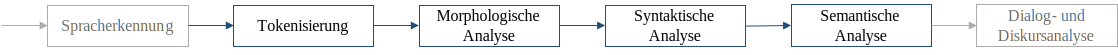
\includegraphics[width=\textwidth]{images/nlp_pipeline_saarbruecken_1line.eps}
	\caption[Saarbrücker Pipeline-Modell]{Darstellung  des Saarbrücker Pipeline-Modells. Die grauen Prozesschritte sind für die Analyse von Tweets nicht notwendig und entfallen daher.}
	\label{img:nlp-pipeline}
\end{figure}


Die \textbf{Spracherkennung} dient dazu, gesprochene Sprache in Textform umzuwandeln. Da die Daten bereits in Textform vorliegen und nicht als Audio-Signal, entfällt dieser Schritt. Bei der \textbf{Dialog- und Diskursanalyse} werden aufeinanderfolgende Sätze und ihre Beziehungen untereinander analysiert. Bei den zu verarbeitenden Daten handelt es sich in der Regel nur um einzelne (oder sehr wenige) Sätze, die nicht in komplexen Beziehungen zueinander stehen. Daher wird auf diesen Schritt verzichtet.


%%% 3.1.1: Tokenisierung  -------------------------------------------------------------------------------------------------------------%
\subsection*{Tokenisierung}
\label{subsec:tokenisierung}
Bei der Tokenisierung wird ein als Zeichenkette vorliegender Text auf Wortebene segmentiert. Ein \textit{Token} ist dabei eine Instanz einer Zeichenfolge, die als semantische Einheit für die Weiterverarbeitung zusammengefasst wurde\footnote{Vgl. \citet{manning2008}, S. 22.}. Bei der Verarbeitung menschlicher Sprache werden die Begriffe \textit{Token} und \textit{Wort} oft synonym verwendet. Eine einfache Form der Tokenisierung ist die sog. White-""Space-""Tokenisierung, bei der der Text an Satz- und Leerzeichen getrennt wird. Es existieren allerdings auch komplexere Tokenizer, die beispielsweise mit regulären Ausdrücken\footnote{Reguläre Ausdrücke sind eine formale Sprache, die zur Beschreibung von Mengen von Zeichenketten mit syntaktischen Regeln dienen.} arbeiten. Solche komplexeren Tokenizer sind notwendig, da nicht in allen Schriftsprachen eine White-""Space-""Tokenisierung möglich ist. Die japanische und chinesische Schrift verwenden beispielsweise keine Leerzeichen zwischen einzelnen Wörtern.\\

Die in der Praxis verwendeten Tokenizer arbeiten oft in zwei Stufen. In der ersten Stufe wird ein vorliegender Text in einzelne Sätze geteilt. Dabei werden verschiedene Methoden verwendet, deren Effizienz stark vom Anwendungsfall abhängt. So nutzt der in der Implementierung verwendete \textit{Punkt-""sentence-""Tokenizer}\footnote{Vgl. \citet{kiss2006}, S. 488 ff.} beispielsweise unüberwachtes Lernen, um aus einem großen Textkorpus einer Sprache eine Sammlung von Abkürzungen, Redewendungen und Satzanfängen zu erstellen, mit der er schließlich Sätze trennen kann. Der Tokenizer ist damit unabhängig von der verwendeten Sprache einsetzbar, sofern ein ausreichender Textkorpus für das Training vorhanden ist. Die zweite Stufe des Tokenizers unterteilt den Satz schließlich in einzelne Tokens. Die Implementierung verwendet dabei eine Menge regulärer Ausdrücke, um zum Beispiel Satzzeichen zu erkennen und Kontraktionen zu trennen (["`We'll"'] $\rightarrow$ ["`We"'], ["`'ll"']).\\


In einem weiteren Schritt wird anschließend jedem Token des Textes eine Wortart, der \textit{part-of-speech} (POS), basierend auf der Definition des Wortes und den angrenzenden Wörtern hinzugefügt. Dafür benötigt der POS-Tagger ein sog. \textit{Tagset}, also eine Menge von Abkürzungen (den \textit{Tags}) für die verschiedenen Wortarten. Für die englische Sprache ist das \textit{Penn Treebank Tagset}\footnote{Vgl. \citet{marcus1993}, S. 317.} weit verbreitet -- für die deutsche Sprache hat sich das Stuttgart-Tübingen Tagset\footnote{Vgl. \citet{schiller1995}.} (STTS) als Standard etabliert.

\begin{figure}[hbt!]
	\centering
	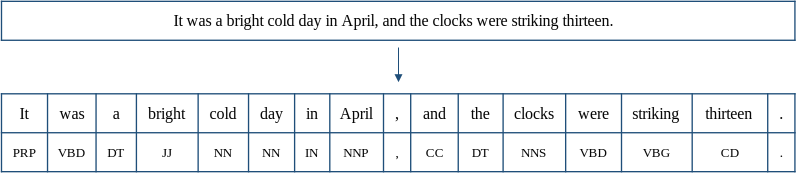
\includegraphics[width=.9\textwidth]{images/nlp_tokenization_example_1984.eps}
	\caption[Beispiel einer Tokenisierung mit POS-Tagging]{Beispiel einer Tokenisierung mit POS-Tagging (PRP = Personalpronomen, JJ = Adjektiv, ...)\footnotemark}
	\label{img:nlp-tokenization-example}
\end{figure}
\footnotetext{Eine vollständige Auflistung der POS-Tags findet sich in Anhang \ref{app:pos-tagsets}.}

Der in der Implementierung verwendete POS-Tagger basiert auf dem Perzeptron-""Algorithmus\footnote{Vgl. \citet{rosenblatt1958}.}, einer vereinfachten Form eines neuronalen Netzes. Die Ausgabe des Perzeptrons ist dabei der gesuchte POS aus dem Penn Treebank Tagset. Das Perzeptron wurde mit verschiedenen Textkorpora trainiert (u.a. Artikel des \textit{Wall Street Journals}, Nachrichten verschiedener Nachrichtenagenturen sowie verschiedene Internet-Quellen wie Blogs, Webseiten und Social Media.).



%%% Morphologische Analyse
\subsection*{Morphologische Analyse}
In der morphologischen Analyse wird versucht, Flexionen von Wörtern zu identifizieren und sie auf ihre Grundform zurückzuführen - das \textit{Lemma}.\\

\begin{Definition}[Lemma]
    Ein \textbf{Lemma} ist die Grundform oder kanonische Form eines Wortes, unter der ein Begriff in einem Nachschlagewerk vorzufinden ist.
\end{Definition}

Ein Lemma ist also die Grundform eines Wortes ohne Deklinationen, Konjugationen oder andere Flexionen, also z. B. Verben im Infinitiv, Substantive im Singular etc. Aufgabe der morphologischen Analyse ist die Rückführen jedes Wortes auf das entsprechende Lemma. In der Praxis kommen dabei zwei verschiedene Verfahren zur Anwendung: Die \textit{Stamm\-form\-reduktion} und die \textit{Lemmatisierung}.
Das heuristische Verfahren der Stamm\-form\-reduktion versucht Wortendungen zu entfernen und dadurch Wörter auf ihre Grundformen zurückzuführen. 
Die Lemmatisierung hingegen nutzt Wörterbücher und morphologische Analysemethoden für die Rückführung auf ein gemeinsames Lemma, indem flexierte Wortteile verändert oder entfernt werden.
Die Lemmatisierung ist der Stammformreduktion dabei hinsichtlich der Genauigkeit überlegen, was insbesondere darauf zurückzuführen ist, dass die Lemmatisierung bei der Analyse umfangreichere Daten wie zum Beispiel Synonyme einbeziehen kann\footnote{Vgl. \citet{balakrishnan2014}, S. 178.}.\\

\begin{figure}[hbt!]
	\centering
	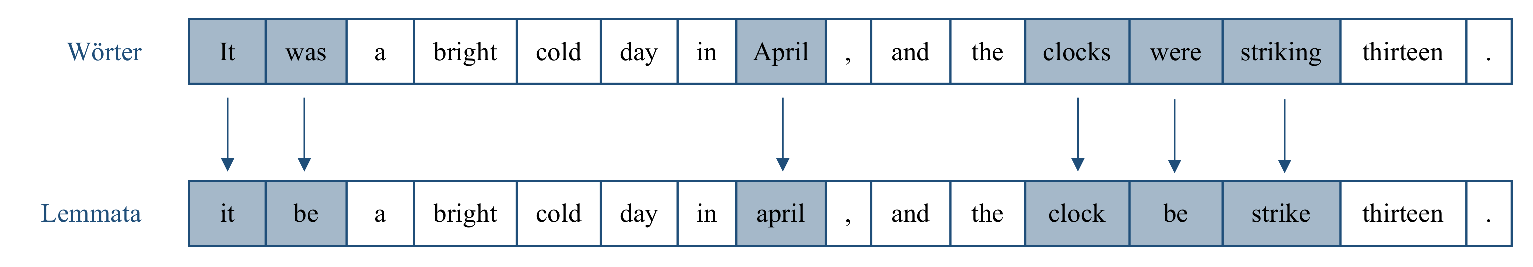
\includegraphics[width=\textwidth]{images/nlp_morphology_example_1984.eps}
	\caption[Beispiel einer Morphologischen Analyse mittels Lemmatisierung]{Beispiel einer Morphologischen Analyse mittels Lemmatisierung. Die durch Lemmatisierung veränderten Worte sind farblich markiert. Alle Worte liegen nach der Lemmatisierung in ihrer Grundform vor: Verben im Infinitiv, Substantive im Nominativ Singular etc.}
	\label{img:nlp-morphology-example}
\end{figure}

Die Implementierung verwendet den \textit{WordNet Lemmatizer}, einen lexikonbasierten Lemmatisierer auf Basis von \textit{WordNet}, einer umfangreichen lexikalischen Datenbank englischer Wörter\footnote{Vgl. \citet{soergel1998}.}. Der Lemmatisierer versucht, ein Lemma in WordNet zu finden. Wenn kein direkter Treffer möglich ist, werden solange Umformungsregeln angewendet, bis ein entsprechendes Lemma in WordNet gefunden wurde, auf das das Wort zurückgeführt werden kann. Dabei sind sowohl das Lexikon (WordNet) als auch das Regelwerk sprachabhängig. Für die deutsche Sprache existiert mit \textit{GermaNet}\footnote{Vgl. \citet{kunze2002}.} ein ähnliches Projekt.



%%% 3.1.3: Syntaktische Analyse  ------------------------------------------------------------------------------------------------------%
\subsection*{Syntaktische Analyse}
Die Ausgabe aus der Lemmatisierung behandelt bisher nur einzelne Wörter bzw. Lemmata und setzt diese nicht in Relation zueinander. Dies ist die Aufgabe eines \textit{Parsers} in der syntaktischen Analyse. Dieser zerlegt einen Satz in seine grammatikalischen Bestandteile und weist jedem Wort eine Funktion im Satz (Subjekt, Prädikat, Objekt, ...) zu. Die einzelnen Worte werden somit hinsichtlich ihrer grammatikalischen Beziehungen zueinander analysiert.\\

Für die syntaktische Analyse eines Satzes wird eine \textit{formale Grammatik} benötigt. Darunter versteht man eine vollständige Liste eindeutiger, formalisierter Regeln zur Bildung von Sätzen\footnote{Die Regeln dienen eigentlich der Bildung von Wörtern (im Sinne der theoretischen Informatik als Folge von Symbolen eines Alphabets), wobei ein Wort in der theoretischen Informatik einem Satz in der deutschen Sprache entspricht. Im Folgenden wird statt dem informatischen "`Wort"' der "`Satz"' verwendet.}. Mit einer formalen Grammatik lassen sich ausgehend von einem Startsymbol $S$ die (Produktions-)Regeln anwenden, um einen Satz zu erzeugen. Die Anwendung einer Regel wird als \textit{Ableitung} bezeichnet. Die Symbole links der Ableitung unterscheidet man in \textit{Terminalsymbole} $T$ und \textit{Nichtterminalsymbole} $N$. Dabei werden solange Regeln angewendet, bis keine Nichtterminalsymbole mehr vorliegen. Beispiel \ref{bsp:cf-grammar} zeigt eine \textit{kontextfreie Grammatik}\footnote{Dabei handelt es sich um einen Spezialfall einer Grammatik, bei der jede Regel genau ein Nichtterminalsymbol auf beliebige andere Symbole ableitet.} und Erläuterungen zu den einzelnen Regeln. \\

\begin{Definition}[Grammatik\footnotemark]
    \label{def:grammatik}
    Eine \textbf{formale Grammatik} ist ein 4-Tupel $G = (V, \ T, \ P, \ S)$ mit
    \begin{itemize}
        \item einem Vokabular $V$
        \item einer Teilmenge $T \subset V$ von Terminalsymbolen
        \item einer Menge $P$ von Produktionsregeln
        \item einem Startsymbol $S \in V \setminus T$
    \end{itemize}
    Die Menge der Nichtterminalsymbole ergibt sich damit durch $N = V \setminus T$.
\end{Definition}
\footnotetext{Vgl. \citet{hromkovic2011}, S. 353.}

Beispiel \ref{bsp:cf-grammar} zeigt, wie man unter Anwendung der Produktionsregeln einen Satz erzeugen kann. Selbst mithilfe der gegebenen Grammatik kann jedoch eine Vielzahl von Sätzen erzeugt werden, wobei jeder Satz grammatikalisch korrekt ist, aber nicht unbedingt inhaltlich richtig oder sinnvoll sein muss. So kann zum Beispiel der Satz "`The cat sat the dog."' erzeugt werden, der nur wenig Sinn ergibt. Die "`Ableitungsgeschichte"'\footnote{Als "`Ableitungsgeschichte"' wird die Folge von Anwendungen der Produktionsregeln (Ableitungen) bezeichnet.} des Satzes kann (wie in Abbildung \ref{img:parse-tree}) als Baumdiagramm (sog. "`parse tree"') dargestellt werden. \\
\bigskip

\begin{Beispiel}[Anwendung einer kontextfreien Grammatik]
    \label{bsp:cf-grammar}
    \begin{tabular}{| p{1cm} p{5cm} |}
    \hline
         (1) & $S$ $\rightarrow$ $NP$ $VP$ \\
         (2) & $PP$ $\rightarrow$ $P$ $NP$ \\
         (3) & $NP$ $\rightarrow$ $Det$ $N$ | $NP$ $PP$ \\
         (4) & $VP$ $\rightarrow$ $V$ $NP$ | $NP$ $PP$ \\
         (5) & $Det$ $\rightarrow$ 'a' | 'the' \\
         (6) & $N$ $\rightarrow$ 'dog' | 'cat' \\
         (7) & $V$ $\rightarrow$ 'chased' | 'sat' \\
         (8) & $P$ $\rightarrow$ 'on' | 'in'\\
         \hline
    \end{tabular}\\
    \smallskip \\
    NP = \textit{noun phrase}, VP = \textit{verb phrase}, PP = \textit{adposition phrase}, | ist als logisches "`oder"' zu verstehen.
    Durch Anwendung der Produktionsregeln lassen sich (beginnend beim Startsymbol $S$) Sätze erzeugen:\\
%    \smallskip
    
    \begin{tabular}{| p{12cm} |}
        \hline
        $S$ \ \ $\xrightarrow{(1)}$ \ \   NP VP\\ \hline
        NP VP \ \ $\xrightarrow{(3),(4)}$ \ \ Det N V NP \\ \hline
        Det N V NP \ \ $\xrightarrow{(3)}$ \ \ Det N V Det N \\ \hline
        Det N V Det N \ \ $\xrightarrow{(5), (6), (7), (5), (6)}$ \ \ "`The dog chased a cat"' \\
        \hline
    \end{tabular}\\
    \smallskip
\end{Beispiel}
\bigskip


\begin{figure}[hbt!]
    \centering
    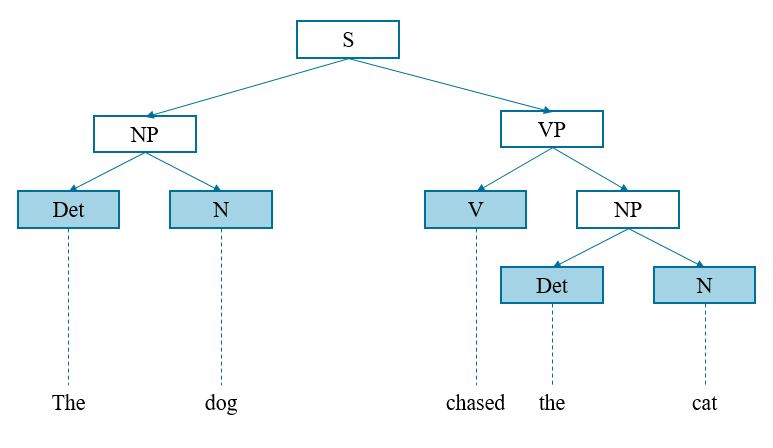
\includegraphics[width=.8\textwidth]{images/grammar_parse_tree.eps}
    \caption[Darstellung eines Parse Trees]{Parse Tree des Satzes aus Beispiel \ref{bsp:cf-grammar}. Die Anwendung einer Produktionsregel (Ableitung) wird durch einen Pfeil nach unten dargestellt.Die letzte Ableitung auf das Terminalsymbol ist als gestrichelte Linie dargestellt und bildet den für Menschen verständlichen Satz\footnotemark.}
    \label{img:parse-tree}
\end{figure}
\footnotetext{Eigene Darstellung.}

Man erkennt an Abbildung \ref{img:parse-tree} auch die sukzessive Zerlegung des Satzes in seine syntaktischen Bestandteile. Die weitere Analyse des Textes kann nun auf unterschiedlichen Ebenen dieser Zerlegung stattfinden. Dazu betrachten wir in der weiteren Analyse die \textit{Phrase} als syntaktische Einheit.\\

\begin{Definition}[Phrase]
    Eine \textbf{Phrase} ist eine abgeschlossene (d.h. syntaktisch gesättigte) syntaktische Einheit.
\end{Definition}

Mit "`syntaktisch gesättigt"' wird in diesem Zusammenhang die Eigenschaft einer Phrase bezeichnet, dass sie alle notwendigen Ergänzungen enthält. Der Begriff ist verwandt mit dem geläufigeren Wort des \textit{Satzglieds}, der einen Spezialfall einer Phrase darstellt. Die semantische bzw. Sentiment-Analyse, wie sie in den nächsten Abschnitten vorgestellt wird, bezieht sich stets auf die Zerlegung eines Satzes in Phrasen, um die vollständige inhaltliche Bedeutung zu erfassen.\\


%%% 3.1.4: Semantische Analyse  -------------------------------------------------------------------------------------------------------%
\subsection*{Semantische Analyse}
Unter dem Begriff der semantischen Analyse wird eine Vielzahl von Analysemethoden zusammengefasst, deren gemeinsames Ziel es ist, die Bedeutung eines Textes zu erfassen. Dazu gehört auch, die mit einem Text verbundene Stimmung im Rahmen einer Sentiment-Analyse zu ermitteln, die im folgenden Abschnitt beschrieben wird.



%%% 3.2: Sentiment-Analyse ------------------------------------------------------------------------------------------------%
\section{Sentiment-Analyse}
\label{sec:sentiment}

Die Sentiment-Analyse ermittelt die in einem Text vermittelte Stimmung des Autors. Anders als bei der \textit{Emotionsanalyse}, bei der spezielle Emotionen wie Freude, Gelassenheit oder Wut identifiziert werden, beschränkt sich die Sentiment-Analyse auf die Analyse der Polarität ("`positiv"' oder "`negativ"') und ggf. der Subjektivität eines Textes.
Einen Text als eindeutig positiv oder eindeutig negativ einzustufen ist (insbesondere für Computer) keine einfache Aufgabe. Es bietet sich daher an, statt einer solchen binären Klassifikation eine stetige Variable auf einem Intervall $[-\omega, \omega]$ einzuführen, um die Polarität abzubilden, wie in Abbildung \ref{img:polarity-scale} dargestellt.

\begin{figure}[hbt!]
	\centering
	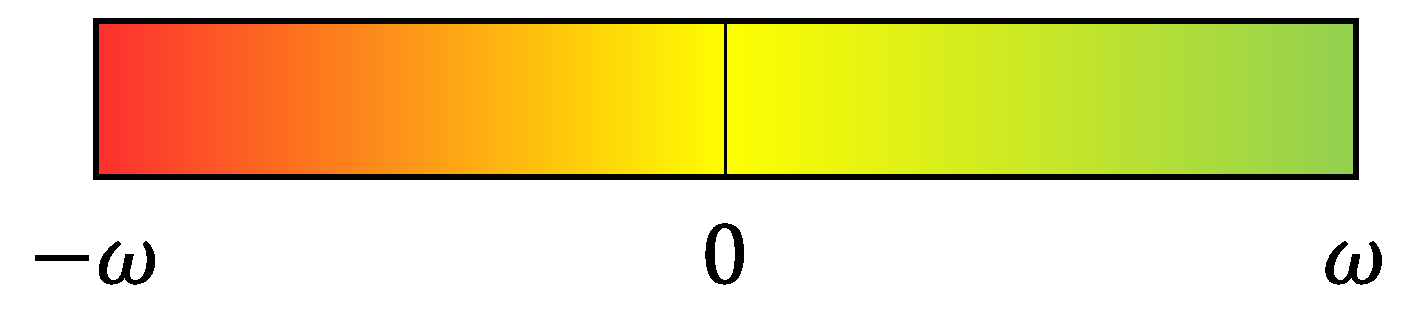
\includegraphics[width=.3\textwidth]{images/polarity_scale.eps}
	\caption[Skala für eine stetige Polaritätsvariable]{Skala für eine stetige Polaritätsvariable\footnotemark.}
	\label{img:polarity-scale}
\end{figure}
\footnotetext{Eigene Darstellung.}

Die Sentiment-Analyse kann damit formal definiert werden:

\begin{Definition}[Sentiment-Analyse]
	\label{def:sentiment-analyse}
	Eine Sentiment-Analyse $A$ für einen Text $T$ eines Textkorpus $\Sigma^*$ ist eine Abbildung	\begin{equation*}
	    A: T \rightarrow [-\omega, \ \omega] \ , \ \ T \in \Sigma^*,
	\end{equation*}
	welche die Polarität des Textes $T$ widerspiegelt.
\end{Definition}

Aus der Definition erkennt man, dass $A$ nur die Polarität der Texte analysiert. Eine komplexere Analyse unter Einbeziehung der Subjektivität eines Textes ist jedoch ebenso denkbar, wenn man die Zielmenge der Abbildung entsprechend definiert, also:
\begin{equation}
    A: T \rightarrow ([-\omega, \ \omega] \times [-s, \ s])
\end{equation}
mit einer Skala $[-s, s]$ für die Subjektivität. Im Folgenden wird $\omega$ als Variable für einen Polaritätswert verwendet. \\

Um eine solche Abbildung $A$ zu finden gibt es zahlreiche Ansätze. In jüngerer Zeit werden vermehrt Methoden des maschinellen Lernens verwendet, um Texte zu analysieren\footnote{Vgl. \citet{boiy2009}.}. "`Klassische"' Methoden verwenden hingegen meist ein Lexikon mit besonderen "`emotionalen Wörtern"', also Wörtern, die eindeutig einem Polaritätswert $\omega$ zugeordnet werden können. Beide Verfahren erreichen in Vergleichsstudien\footnote{Vgl. \citet{dhaoui2017}, S. 14 und \citet{kolchyna2015}, S. 11 ff.} ähnliche durchschnittliche Genauigkeitswerte, jedoch hängt die Genauigkeit stark vom speziellen Anwendungsfall ab. Im folgenden Abschnitt wird ein Ansatz für ein solches \textit{lexikonbasiertes Verfahren} vorgestellt.
\clearpage


%%% 3.2.1: Lexikonbasierte Verfahren ------------------------------------------------------------------------------------- %
\subsection*{Lexikonbasierte Verfahren}
\label{subsec:lexicon-based}

Lexikonbasierte Verfahren ermitteln das Sentiment eines Textes unter Verwendung eines \textbf{Lexikons} mit Lemmata und deren zugehörigen Polaritätswerten, die unter Verwendung eines \textbf{Regelwerkes} angewendet werden. Schließlich wird für den Text ein \textbf{Gesamtsentiment} aus den einzelnen Sentiments ermittelt.\\

%%% 3.2.1.1: Das Lexikon
\subsubsection*{Das Lexikon}
Lexikonbasierte Verfahren berechnen ein Gesamtsentiment eines Textes auf Basis der einzelnen Lemmata der Wörter im Text\footnote{Vgl. \citet{turney2002}.}. Das dafür verwendete Lexikon kann manuell oder automatisch erzeugt werden\footnote{Vgl. \citet{stone1966}.}.
Bei der manuellen Erzeugung werden in Laborexperimenten von zuvor geschulten Teilnehmern Wörter auf einer Skala (z. B. von -5 bis +5) bewertet\footnote{Vgl. \citet{dodds2010}, S. 442f.}. Die so ermittelten Polaritätswerte jedes Wortes werden unter dem entsprechendem Lemma zusammengeführt. Dabei werden neben den Mittelwerten oft auch die Standardabweichungen der Bewertungen im Lexikon gespeichert. Da die Genauigkeit der Analyse sehr stark von der Qualität des verwendeten Lexikons abhängt, findet oft noch eine Überprüfung des gesamten Lexikons durch eine Gruppe von Experten statt, um die Subjektivität in den Daten zu minimieren\footnote{Vgl. \citet{taboada2011}.}. Abbildung \ref{fig:lexicon} zeigt einen Auszug aus dem Lexikon des \textit{VADER}-SentimentAnalyzers, der in der Implementierung verwendet wurde.\\

Automatisch erzeugte Lexika verwenden oft einen Kern sog. "`seed words"', um daraus ein Lexikon mit positiven bzw. negativen Wörtern aufzubauen. Dafür werden große Textkorpora analysiert und Worte aufgrund der Häufigkeit des gemeinsamen Auftretens (der sog. "`Kookurrenz"') mit den bekannten seed words kategorisiert und dem Lexikon hinzugefügt\footnote{Vgl. \citet{kanayama2006}.}.\\


\begin{figure}[hbt!]
    \centering
    \begin{tabular}{| p{2cm} | p{2cm} | p{2cm} | p{8cm} |}
        \hline
        \rowcolor{tubs_blue_light60}
        \textbf{lemma} & \textbf{avg} & \textbf{st.dev} & \textbf{values} \\
        \hline
        $\vdots$ & $\vdots$ & $\vdots$ & $\vdots$ \\
        hell &  -3.6 & 0.66332 & [-4, -4, -4, -4, -4, -2, -3, -4, -3, -4] \\
        help & 1.7 & 0.78102 & [3, 2, 1, 2, 1, 2, 3, 1, 1, 1] \\
        hero & 2.6 & 0.8 & [2, 3, 2, 2, 4, 4, 2, 3, 2, 2] \\
        heroic & 2.6 & 0.8 & [3, 3, 1, 4, 2, 3, 2, 3, 2, 3] \\
        $\vdots$ & $\vdots$ & $\vdots$ & $\vdots$ \\
				\hline
    \end{tabular}

    \caption[Auszug aus dem Lexikon eines Sentiment-Analyzers]{Auszug aus einem typischen Lexikon, wie es in lexikonbasierten Sentiment-Analyzern verwendet wird. Die Spalte \textit{values} enthält die Beurteilungen der Testpersonen auf einer Skale von $+5$ bis $-5$\footnotemark.}
    \label{fig:lexicon}
\end{figure}
\footnotetext{In Anlehnung an \citet{hutto2014}.}


%%% 3.2.1.2: Das Regelwerk
\subsubsection*{Das Regelwerk}
Der zweite Baustein eines lexikonbasierten Verfahrens ist das Regelwerk. Es besteht aus verschiedenen Regeln, die z. B. \textbf{Verstärkungen} oder \textbf{Negationen} bei der Bewertung eines Textes berücksichtigen.\\

Ein \textbf{Verstärker} verändert die Polarität des Lemmas, auf das er sich bezieht. Meist wird dies durch eine multiplikative Konstante umgesetzt. Das gleiche Schema kann auch auf Adjektiv-Substantiv-Kombinationen angewendet werden. So ist z. B. "`Problem"' weniger negativ konnotiert als "`riesiges Problem"', was ebenfalls mit einer multiplikativen Konstante dargestellt wird. Es gibt jedoch auch Modelle, in denen statt einer multiplikativen eine additive Konstante verwendet wird.\\

Während Verstärker oft in unmittelbarer Nähe ihres Bezugswortes stehen, können \textbf{Negationen} auch weiter entfernt stehen (z. B. "`Nobody gave a good performance in this movie."'). Die richtige computerlinguistische Verarbeitung des Textes ist daher entscheidend, um eine Phrase zu identifizieren und analysieren zu können\footnote{Vgl. \citet{taboada2011}, S. 276.}. Wenn eine Phrase mit Negation erfolgreich erkannt wurde, muss der Polaritätswert des negierten Lemmas entsprechend angepasst werden. Ähnlich wie bei der Verarbeitung der Modifikationen stehen auch hier verschiedene Optionen zur Verfügung:

\begin{itemize}
	\item \textbf{switch negation}: Der Polaritätswert des Lemmas wird umgekehrt, indem er mit $-1$ multipliziert wird
	\item \textbf{shift negation}: Der Polaritätswert wird in Richtung der entgegengesetzten Polarität verschoben, indem z. B. $+4$ (bei einem Lemma mit negativer Polarität) addiert wird
\end{itemize}

Das Beispiel \ref{bsp:modifications} zeigt einige Anwendungen von verschiedenen Verstärkungen und Negationen.

\begin{Beispiel}[Verstärkungen und Negationen]
    \label{bsp:modifications}
    \textbf{Verstärkungen:}\smallskip
    
    \begin{tabular}{| p{4cm} | p{4cm} |}
        \hline
        "`good"' &  $+2$ \\ \hline
        "`very good"' & $+2 \cdot 1,5 = +3$ \\ \hline
        "`somewhat good"' & $+2 \cdot 0,8 = +1,6$ \\ \hline
    \end{tabular}\\
		\smallskip
		
			Durch die Verstärkung "`very"' wird das Lemma "`good"' verstärkt, indem die für den Verstärker "`very"' festgelegte multiplikative Konstante angewendet wird. Der Verstärker (bzw. in diesem Fall "`Abschwächer"') "`somewhat"' wird analog angewendet mit einer multiplikativen Konstante, die kleiner als 1 ist.\\
  
    \textbf{Negationen:}\smallskip
    
    \begin{tabular}{| p{4cm} | p{4cm} | p{4cm} |}
        \hline
        "`good"' &  $+2$ & \ \\ \hline
        "`not good"' & $+2 \cdot (-1) = -2$ & \textit{switch negation} \\ \hline
        "`not good"' & $+2 - 3 = -1$ & \textit{shift negation} \\ \hline
    \end{tabular}\\
		\smallskip
		
		Die switch negation invertiert die Polarität des Lemmas, während bei der shift negation in entgegengesetzter Richtung der Polarität eine Konstante addiert wird. Vorteilhaft bei der shift negation ist z. B. die Stabilität bei mehrfacher Anwendung einer Negation. "`Not not good"' erhält unter der switch negation den gleichen Polaritätswert wie "`good"', was der menschlichen Wahrnehmung dieser Phrase entspricht.\\
    
\end{Beispiel}

Neben einem Lexikon mit Polaritätswerten für die einzelnen Lemmata müssen also auch Lexika für die Verstärker und die Negationswörter und deren zugehörigen Anpassungsregeln, d.h. additive oder multiplikative Kontanten, erstellt werden. Die Wahl des richtigen Regelwerkes kann dabei sehr starke Auswirkungen auf die Genauigkeit der Sentiment-Analyse haben und die richtige Auswahl hängt vom spezifischen Anwendungsfall ab\footnote{Vgl. \citet{liu2009}, S. 162.}.\\


%%% 3.2.1.3: Das Gesamtsentiment
\subsubsection*{Das Gesamtsentiment}


Um mithilfe des vorgestellten Lexikons und des Regelwerks ein Gesamtsentiment für einen Text ermitteln zu können, muss dieser zunächst wie in Abschnitt \ref{sec:nlp-basics} beschrieben vorverarbeitet werden. Anschließend kann die in Definition \ref{def:sentiment-analyse} eingeführte Sentiment-Analyse $A$ auf dem Text durchgeführt werden:\begin{equation}
    A(T) = \sum_{p \in P} A(p)
\end{equation}
wobei $P$ die Menge aller Phrasen des Textes $T$ ist. Die Sentiment-Analyse einer Phrase $A(p)$ kann unter Verwendung von Lexikon und Regelwerk für den Fall multiplikativer Konstanten für Negationen und Verstärker ausgedrückt werden durch:\begin{equation}
    A(p) =\begin{cases}
                        \sum_{i=1}^{n} \omega_i \cdot \prod_{j} n_{i,j} \prod_{k} m_{i,k}   & , \ n \geq 0 \\
                        0 & , \ n = 0
                    \end{cases}
\end{equation}
mit
\begin{itemize}
	  \setlength\itemsep{0.1em}
    \item den Polaritätswerten $\omega_i$ aller Lemmata
    \item den zu $\omega_i$ zugehörigen Negationswörtern $n_{i,j}$
    \item den zu $\omega_i$ zugehörigen Verstärkern $m_{i, k}$ und
    \item der Anzahl der in $p$ enthaltenen Phrasen $n$
\end{itemize}

Bei der Analyse einer Phrase ist es entscheidend, die richtige Ebene der Phrase für die Analyse zu verwenden. Im Baumdiagramm in Abbildung \ref{img:parse-tree} sind beispielsweise mehrere Ebenen von Phrasen für die Analyse verfügbar. Da jedes Lemma nur einfach in das Gesamtsentiment einfließen soll, empfiehlt sich ein einfacher rekursiver Algorithmus für die Sentiment-Analyse einer Phrase:


\begin{lstlisting}[float, language=python, caption={Rekursiver Algorithmus zum Ermitteln der relevanten Phrasenebene}, label={lst:phrase-recursion}]
    def recursive(phrase):
    For alle Phrasen $p$:
      Ermittle parent p' zu p
      If p'\p enthaelt Negation, Verstaerker oder Lemmata
      Then:
        phrase = recursive(phrase)
        return(phrase)
      Else:
        return(phrase)
\end{lstlisting}

Mithilfe des Algorithmus in Quellcode \ref{lst:phrase-recursion} wird die relevante Phrase ermittelt. Wenn die "`Eltern"=Phrase"' $p'$, d.h. die Phrase, die im Baumdiagramm über dem Element $p$ steht, einen Verstärker, eine Negation oder ein Lemma enthält, dann wird für die Sentiment-Analyse die Eltern-Phrase verwendet. Durch die Rekursion wird der Baum solange nach oben durchlaufen bis durch ein weiteres Aufsteigen keine Phrasen mit zusätzlichem Informationsgehalt mehr gefunden werden können.\\

%%% 3.4: Datenbeschaffung ---------------------------------------------------------------------------------------------------%
\section{Datenerhebung}
\label{sec:datenerhebnug}

In den vergangenen Kapiteln wurden die Grundlagen für die Textverarbeitung und Sen\-ti\-ment"=Analy\-se (beliebiger) Texte vorgestellt. Für die praktische Anwendung müssen nun zunächst Daten beschafft und analysiert werden.

%%% 3.4.1
\subsection*{Wahl eines sozialen Mediums}
Die Kommunikation im Internet hat in den letzten Jahren stetig zugenommen. Dabei greifen immer mehr Nutzer auf sogenannte Microblogging-Dienste wie Twitter, Tumblr oder Facebook zurück, um ihre Meinung zu äußern, statt traditionelle internetbasierte Kommunikationsmittel wie E-Mails oder klassische Blogs zu verwenden. Twitter macht dabei mit 330 Millionen aktiven Nutzern\footnote{Vgl. \citet{statista2019}.} und durchschnittlich 500 Mio. Tweets pro Tag einen bedeutenden Anteil dieser Kommunikation aus. Die Wahl von Twitter als Datenquelle für die Analyse ist somit naheliegend. Obwohl die Anzahl der Zeichen je Tweet auf 140\footnote{Im November 2017 wurde die maximale Anzahl der Zeichen von 140 auf 280 Zeichen erhöht.} Zeichen beschränkt ist, liefert Twitter zu nahezu jedem Thema eine große Anzahl an Tweets mit persönlichen Meinungen und ermöglicht daher eine gute Repräsentation der Stimmungslage. Die Verwendung von \textit{hashtags} ermöglicht darüber hinaus eine einfache Gruppierung von Tweets zu einem bestimmten Thema.



%%% 3.4.2
\subsection*{Twitter-API}
Daten können von Twitter durch die Twitter""-Programmierschnittstelle (engl. \textit{application programming interface, API}) abgerufen werden. Twitter stellt dabei neben einer Streaming-API für Echtzeitdaten auch die hier verwendete REST\footnote{Representational State Transfer (REST)}-API für historische Daten zur Verfügung\footnote{Vgl. \citet{pfaffenberger2016}, S. 54f.}. Teil dieser REST-API ist die \textit{Search API}, mit der die historischen Tweets abgerufen werden können. An diese API kann ein HTTP\footnote{Hypertext Transfer Protocol}-Request gesendet werden. Dieser muss neben den Zugangsdaten - Twitter nutzt das Open Authorization (OAuth)-Protokoll für die Autorisierung - eine gültige Query enthalten. Diese besteht aus den verschiedenen Suchparametern (Datum bzw. Datumsbereich, Suchbegriff, Hashtag, Nutzername etc.), nach denen die Tweets gefiltert werden sollen. Die HTTP-Response enthält schließlich alle der Query entsprechenden Tweets im JSON-Format\footnote{JavaScript Object Notation (JSON)}.\\


%%% 3.4.3
\subsection*{Speicherung der Daten}
\label{subsec:saving-data}
Die Twitter-API stellt eine Sammlung von Tweets im JSON-Format zur Verfügung. Die Struktur dieses Dateityps erlaubt eine einfach lesbare Textform bei gleichzeitiger starker Komplexität der Daten, indem mittels Verschachtelungen Werte zu Gruppen zusammengefasst oder durch Verwendung von Arrays auch umfangreiche Datenmengen gespeichert werden können. Ein einzelner Tweet, wie er von der API zurückgegeben wird, enthält viele Informationen, die für die weitere Analyse nicht notwendig sind. Um den Speicherbedarf zu reduzieren werden überflüssige Informationen daher zunächst entfernt. Dadurch kann der Speicherbedarf eines einzelnen Tweets um mehr als 90\% reduziert werden (von durchschnittlich $4,2$kB auf ca. $400$kb). \\

\begin{figure}[hbt!]
	\centering
	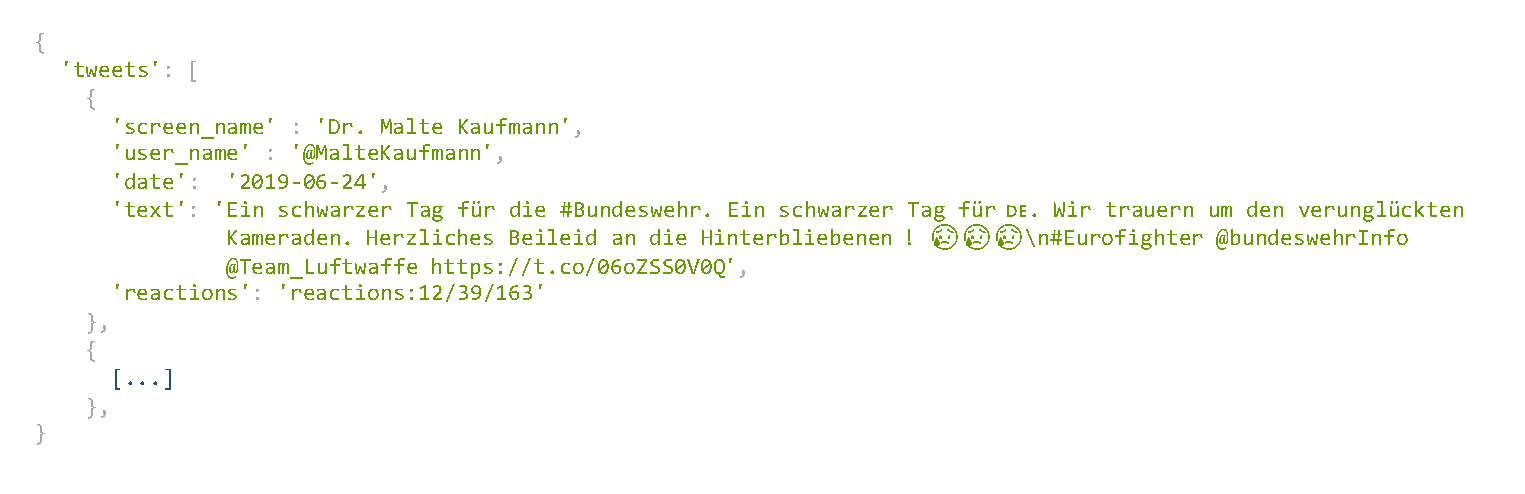
\includegraphics[width=.9\textwidth]{images/reduced_tweet_json.eps}
	\caption[Beispiel eines Tweets im reduzierten Format]{Beispiel eines Tweets im reduzierten Format. Die überflüssigen Meta-Informationen (z. B. Betriebssystem des Nutzers oder sein Profilbild) wurden entfernt\footnotemark.}
	\label{img:json-example-tweet-reduced}
\end{figure}
\footnotetext{Eigene Darstellung.}

Für die Speicherung der Daten wird eine SQLite-Datenbank verwendet. In Abbildung \ref{img:data-model} ist das Datenmodell für die Speicherung der Tweets dargestellt. Die Abbildung zeigt auch die übrigen Tabellen der Datenbank für die Speicherung der einzelnen Suchanfragen, die an die API gesendet wurden, und für die Speicherung der Aktienkurse für die spätere Regressionsanalyse. Die Datenbank und die im Datenmodell beschriebenen Tabellen können mit den Funktionen aus Anhang \ref{subsec:create-tables} erzeugt werden. \\

\begin{figure}[hbt!]
	\centering
	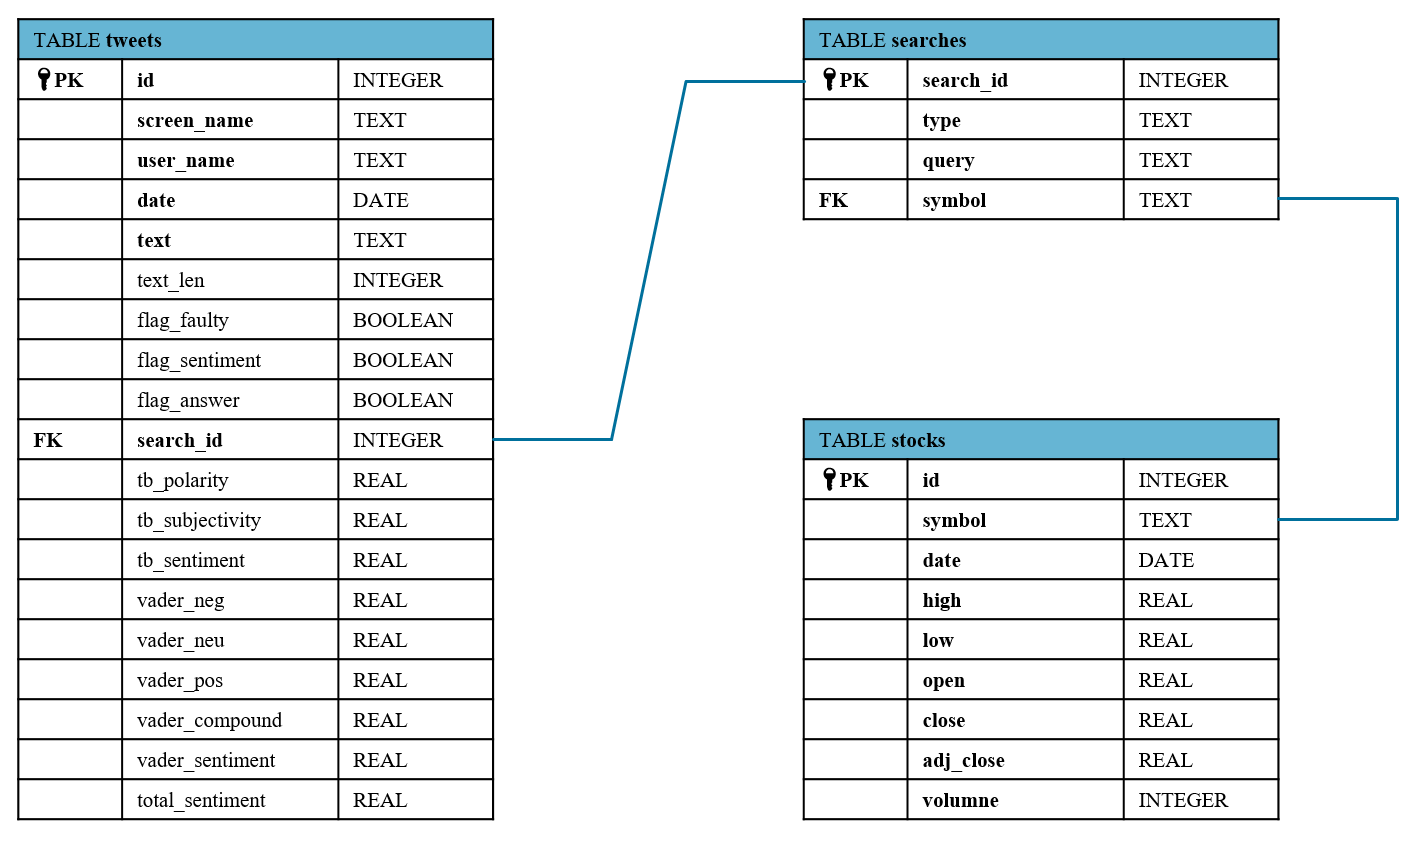
\includegraphics[width=.9\textwidth]{images/data-model.eps}
	\caption[Datenbank-Modell zur Speicherung der Daten]{Datenbank-Modell zur Speicherung der Daten für die Regressionsanalyse\footnotemark}
	\label{img:data-model}
\end{figure}
\footnotetext{Eigene Darstellung.}


%%% 3.4: Implementierung ---------------------------------------------------------------------------------------------------%
\section{Implementierung}
Die Implementierung erfolgt in der Programmiersprache \textit{Python}. Die Schritte des NLP wurden dabei mit dem Paket \textit{NLTK} umgesetzt. Die Sentiment-Analyse basiert auf dem Paket \textit{VADER}.


%%% 3.4.1: NLP ------------------------------------------------------------------------------------- %
\subsection*{Natural Language Toolkit (NLTK)}


%%% 3.4.1.1: Tokenisierung
\subsubsection*{Tokenisierung}
Der Tokenizer des NLTK-Paketes arbeitet wie in Abschnitt \ref{subsec:tokenisierung} beschrieben in zwei Stufen. Die Funktion \textit{word\_tokenize} verwendet zunächst die Funktion \textit{sent\_tokenize}, um einen Text in einzelne Sätze zu zerteilen. Anschließend wird jeder Satz mit \textit{word\_tokenize} in die einzelnen Tokens zerlegt. Abbildung \ref{lst:python-tokenize} zeigt einen exemplarischen Aufruf der beiden Funktionen.

\lstinputlisting[language = Python,
                 label = {lst:python-tokenize},
                 caption = {Tokenisierungs-Funktionen des NLTK-Paketes},
                 ]
                 {code/tokenize.py}


Der auf dem Perzeptron-Algorithmus basierende POS-Tagger kann mit der Funktion \textit{pos\_tag} aufgerufen werden. Dafür muss der Text bereits in tokenisierter Form vorliegen.

\lstinputlisting[language = Python,
                 label = {lst:python-pos-tag},
                 caption = {POS-Tagger des NLTK-Paketes},
                 ]
                 {code/tokenize.py}

\clearpage
%%% 3.4.1.2: Morphologische Analyse
\subsubsection*{Morphologische Analyse}
Der WordNet-Lemmatizer des NLTK-Paketes verwendet das Lexikon \textit{WordNet} und kann wie in Quellcode \ref{lst:python-lemmatize} dargestellt aufgerufen werden.

\lstinputlisting[language = Python,
                 label = {lst:python-lemmatize},
                 caption = {Lemmatisierer des NLTK-Paketes auf Basis von WordNet},
                 ]
                 {code/lemmatize.py}


%%% 3.4.1.3 Syntaktische Analyse
\subsubsection*{Syntaktische Analyse}
Das im folgenden Abschnitt verwendete Paket zur Sentiment-Analyse verwendet im Gegensatz zu anderen Modellen einen in die Sentiment-Analyse integrierten Algorithmus zur syntaktischen Analyse. Auf eine gesonderte syntaktische Analyse kann daher verzichtet werden.\\



%%% 3.5.2: VADER ------------------------------------------------------------------------------------- %
\subsection*{VADER}
Mit dem \textit{\textbf{V}alence \textbf{A}ware \textbf{D}ictionary and s\textbf{E}ntiment \textbf{R}easoner} (VADER) existiert ein lexikonbasiertes Python-Paket für die Sentiment-Analyse, das im Vergleich zu anderen Paketen über ein sehr komplexes Regelwerk verfügt. Es wurde speziell für die Analyse von Texten aus sozialen Netzwerken entwickelt. Die Entwickler von VADER, Hutto und Gilbert, konnten zeigen, dass ihre Kombination von Lexikon und Regeln auf Texten aus sozialen Netzwerken besonders präzise arbeitet und sogar "`menschliche Klassifikatoren"' bei der binären Klassifikation von Tweets übertrifft\footnote{Vgl. \citet{hutto2014}, S. 8.}.\\

Um das Regelwerk aufzustellen, wurden zunächst von zwei Linguistik-Experten ein Korpus von 800 Tweets manuell analysiert, wobei jedem Tweet ein Sentiment von $-4$ bis $+4$ zugewiesen wurden. Anschließend wurden aus den Daten fünf Heuristiken abgeleitet:
\begin{enumerate}
    \item Interpunktion (insbesondere das Ausrufezeichen) hat einen starken Einfluss auf die Intensität des Sentiment
    \item Großschreibung ganzer Wörter verstärkt die Intensität eines Sentiments
    \item Verstärker verstärken die Intensität des Sentiments
    \item Konjunktionen wie "`aber"' signalisieren einen Wechsel der Stimmung, wobei das Gesamtsentiment maßgeblich vom der Konjunktion folgenden Satz abhängt
    \item Ein Großteil (ca. 90\%) der negierten Phrasen kann durch das Trigramm\footnote{Als Trigramm wird ein Satzfragment von drei aufeinanderfolgenden Wörtern bezeichnet.} identifiziert werden, das einem Lemma vorausgeht 
\end{enumerate}

Die so gewonnenen Regeln wurden anschließend getestet, indem 20 Testpersonen die zuvor von Experten analysierten Tweets mit leichten Modifikationen (z. B. mit veränderter Interpunktion) vorgelegt wurden. Aufgrund der so gewonnenen Daten konnten die Regeln quantifiziert und in das Regelwerk implementiert werden.\\

Das von VADER verwendete Lexikon basiert auf zahlreichen bereits bestehenden Lexika. Dabei wurden ca. $7.500$ Lemmata identifiziert, die besonders für den Bereich von Texten aus sozialen Netzwerken geeignet sind. Darunter befinden sich auch zahlreiche Worte aus dem "`Netzjargon"', (z. B. "`LOL"', "`ROFL"') sowie Emoticons. Zusammen mit dem aufgestellten Regelwerk konnte so ein Modell für die Sentiment-Analyse entwickelt werden.\\


\begin{figure}[hbt!]
    \centering
    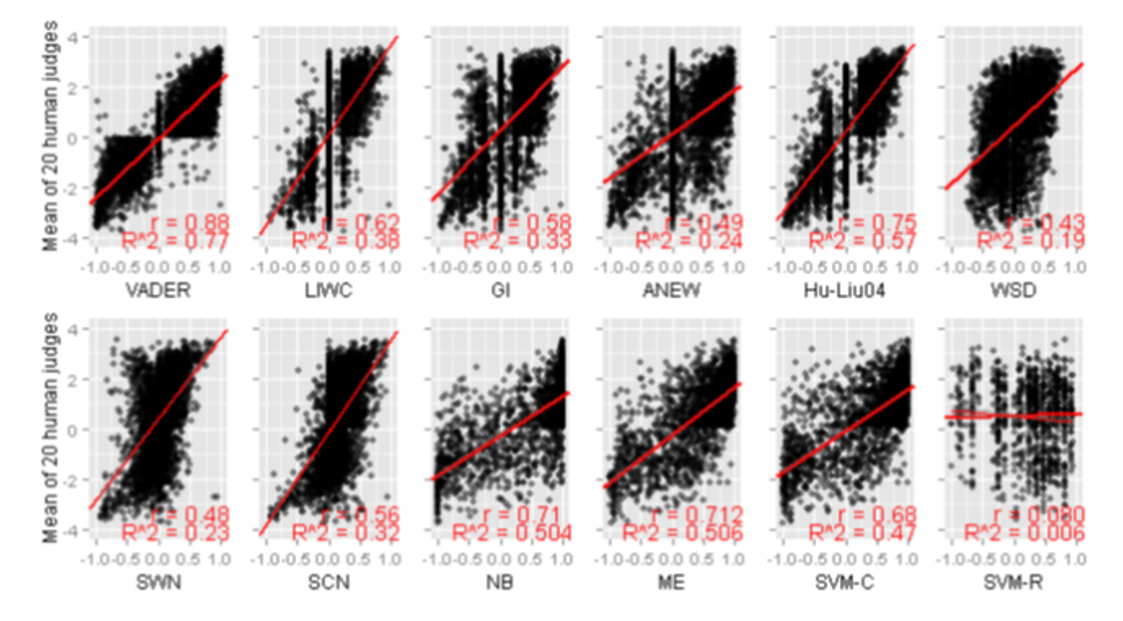
\includegraphics[width=.9\textwidth]{images/vader_comparison.eps}
    \caption[Sentiment-Werte verschiedener Sentiment-Analyse-Tools im Vergleich]{Sentiment-Werte verschiedener Sentiment-Analyse-Tools\footnotemark}
    \label{fig:vader-comparison}
\end{figure}
\footnotetext{Aus: \citet{hutto2014}, S. 8.}

Dieses Modell wurde anschließend mit 11 anderen Sentiment-""Analyse-""Modellen auf einen Korpus von ca. 4.000 Tweets angewendet und die ermittelten Sentiments mit denen der menschlichen Testpersonen verglichen. Abbildung \ref{fig:vader-comparison} zeigt die hohe Genauigkeit von VADER im Vergleich zu anderen Modellen. Insbesondere der geringe Anteil von falsch negativen (linker oberer Quadrant im Diagramm) und falsch positiven (rechter unterer Quadrant im Diagramm) Klassifikationen fällt dabei auf. Zum Vergleich der Gesamtgenauigkeit der Modelle wurde das \textit{F-Maß}\footnote{Definition in Anhang \ref{sec:definitions}.} verwendet. Bei der Analyse von Tweets konnte VADER mit einem $F_1$-Maß von $F_{1, VADER} = 0,96$ alle anderen getesteten Modelle sowie individuelle menschliche Testpersonen ($F_{1, human} = 0,84$) übertreffen.\\

In Python ist das gesamte VADER-Modell in einem Paket implementiert\footnote{Vgl. \citet{vader}.}. Mit der \textit{SentimentIntensityAnalyzer}-Klasse kann eine Phrase durch den Aufruf der Funktion \textit{polarity\_scores} (wie in Quellcode \ref{lst:python-vader} dargestellt) analysiert werden. Für die Analyse größerer Mengen von Tweets findet sich in Anhang \ref{lst:python-vader-sql-batch} eine Funktion, die eine Menge von Tweets abruft, analysiert und an die Datenbank zurückgibt.

\lstinputlisting[language = Python,
                 label = {lst:python-vader},
                 caption = {Python: Sentiment-Analyse des VADER-Paketes},
                 ]
                 {code/vader.py}
                 




%%% 3.6: Ergebnis  --------------------------------------------------------------------------------------------------------%
\section{Ergebnis}
Mit den in Abschnitt \ref{sec:datenerhebnug} vorgestellten Methoden wurde eine Datenbank erzeugt und mit den abgerufenen Tweets gefüllt. Dabei wurden exemplarisch verschiedene Unternehmen in unterschiedlichen Zeiträumen betrachtet. Tabelle \ref{tab:datasets} enthält eine Übersicht der erzeugten Datensätze. Insgesamt wurden $343.674$ Tweets abgerufen, von denen $212.599$ analysiert und verwendet werden konnten.\\


\begin{table}[hbt!]
    \centering
		\begin{tabular}{| p{2.3cm} | p{5.7cm} | p{4.5cm} | p{1.5cm} |}
				\hline
				\rowcolor{tubs_blue_light60}
				\textbf{Datensatz} & \textbf{Query} & \textbf{Zeitraum} & \textbf{Tweets} \\
				\hline
				TESLA1819 & \#tesla,@tesla & 01.01.2018 - 31.12.2019 & 78.489 \\
				MSFT18 & \#microsoft,@microsoft & 01.01.2018 - 31.12.2018 & 29.545 \\
				SIEMENS19 & \#siemens,@siemens,siemens & 01.01.2019 - 31.12.2019 & 21.987 \\
				NESTLE19 & \#nestle,@nestle & 01.01.2019 - 31.12.2019 & 62.795 \\
				DBK19 & \#DeutscheBank,@DeutscheBank & 01.01.2019 - 31.12.2019 & 19.783 \\
				EXXON18 & \#Exxon,@exxonmobil,exxon & 01.01.2018 - 31.12.2018 & 22.215 \\
				\hline
		\end{tabular}
    \caption[Übersicht über die erzeugten Datensätze]{Übersicht über die erzeugten Datensätze\footnotemark}
    \label{tab:datasets}
\end{table}
\footnotetext{Eigene Darstellung.}

Aus diesen Daten muss nun eine Zeitreihe erzeugt werden, die in der Regressionsanalyse mit den Aktienkursen verglichen werden kann. Da die Aktienkurse tagesweise verfügbar sind, liegt es nahe, die Sentiment-Daten ebenfalls tagesweise zu aggregieren. Für jeden Tag eines Zeitraums wird daher der Mittelwert der Sentiments aller Tweets ermittelt. Dabei werden als fehlerhaft klassifizierte Tweets nicht berücksichtigt. Ebenso werden Tweets mit einem Sentiment von $0$ nicht einbezogen, da bei diesen in der Regel kein richtiges Sentiment ermittelt werden konnte (z. B. da keine Lemmata mit Polaritätswerten vorhanden waren). Die Aggregation der Daten auf Tagesebene und die Verknüpfung mit den Aktienkursen ist in Quellcode \ref{lst:sql-get-full-timeseries} umgesetzt. \\

Abbildungen \ref{fig:timeseries-xom} und \ref{fig:timeseries-tsla} zeigen die Zeitreihen von zwei der erzeugten Datensätze. Man erkennt die unterschiedlichen Niveaus des Sentiments ($\mu_{sent}(\text{TSLA}) = 0,28$, $\mu_{sent}(\text{XOM}) = 0,09$), d.h. die Tweets über Tesla sind durchschnittlich deutlich positiver als die Tweets über Exxon Mobil.
Insbesondere bei den Ausreißern in den Zeitreihen lässt sich durch bloße Betrachtung eine Korrelation vermuten, z.B. bei Exxon Mobil im Februar 2018. Die stark gestiegene Anzahl der Tweets ging hier mit einem steigenden Sentiment und einem fallenden Aktienkurs einher.\\


\begin{figure}[hbt!]
    \centering
    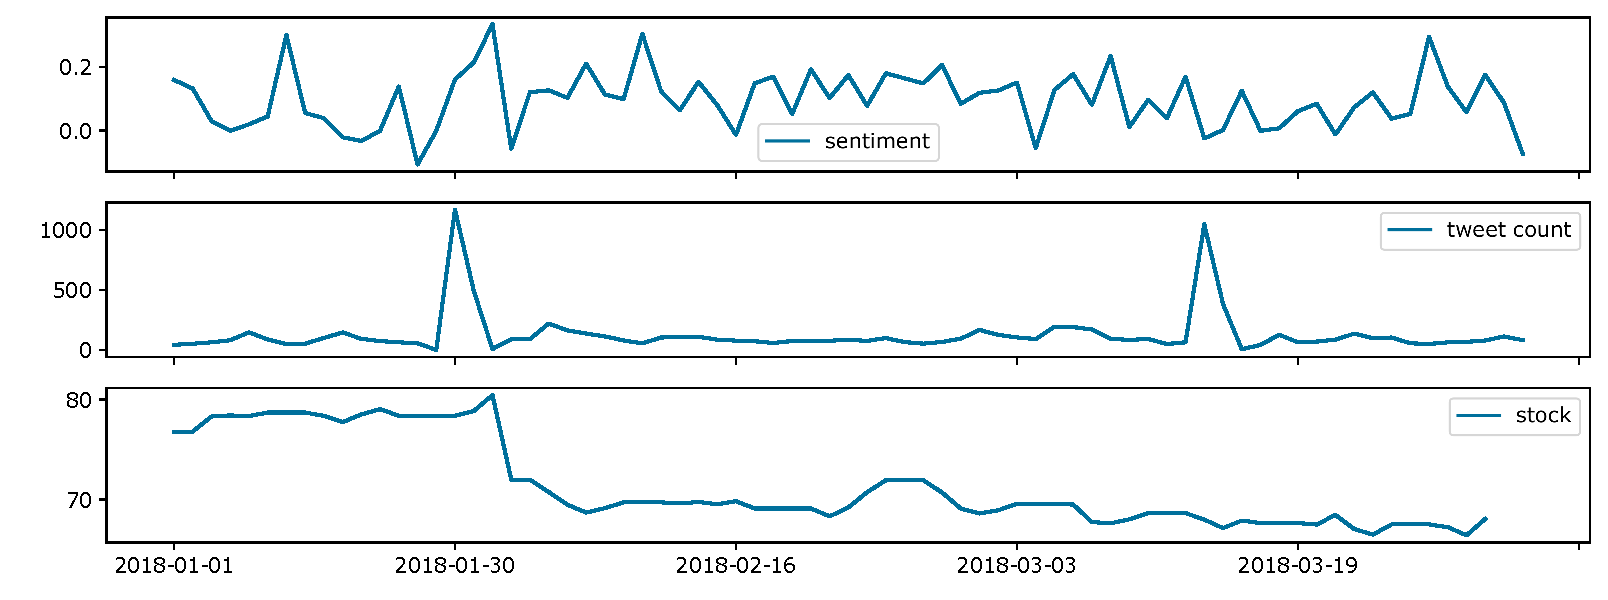
\includegraphics[width=\textwidth]{images/timeseries_XOM_3M.eps}
    \caption[Zeitreihen der Exxon Mobil, 3 Monate]{Zeitreihen der Exxon Mobil (Sentiment-Werte, Anzahl der Tweets, Aktienkurs) über einen Zeitraum von 3 Monaten\footnotemark.}
    \label{fig:timeseries-xom}
\end{figure}
\footnotetext{Eigene Darstellung.}


\begin{figure}[hbt!]
    \centering
    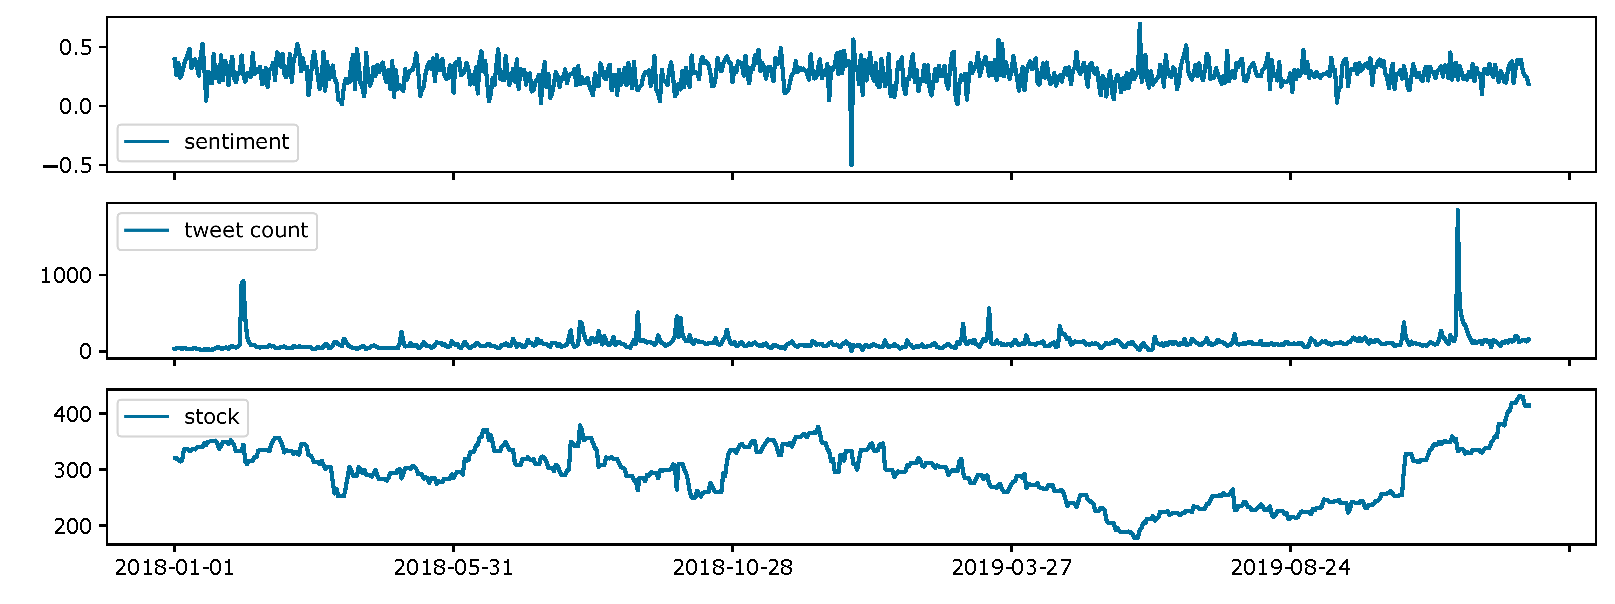
\includegraphics[width=\textwidth]{images/timeseries_TSLA_2Y.eps}
    \caption[Zeitreihen der Tesla, Inc., 2 Jahre]{Zeitreihen der Tesla, Inc. (Sentiment-Werte, Anzahl der Tweets, Aktienkurs) über einen Zeitraum von 2 Jahren.\footnotemark}
    \label{fig:timeseries-tsla}
\end{figure}
\footnotetext{Eigene Darstellung.}

Die Visualisierung der Zeitreihen und die Ermittlung einiger statistischer Werte kann mit der Funktion \textit{get\_dataset\_statistics} erzeugt werden, die in \ref{lst:python-dataset-statistics} beschrieben ist.




% ------------------------------------------------------------------------------------------------------------------------ %
%%% Kapitel 4: Analyse und Prognose von Kursentwicklungen
% ------------------------------------------------------------------------------------------------------------------------ %
\chapter{Regressionsanalyse und Prognose von Kursentwicklungen}
Bei einfacheren Regressionen (z. B. linearen Regressionen) wird von vornherein eine Unterscheidung zwischen endogenen und exogenen Variablen getroffen. Ein vektorautoregressives Modell (VAR) hingegen trifft diese Unterscheidung nicht -- alle Variablen werden als abhängige (endogene) Variablen gleich behandelt.
Ähnlich wie bei univariaten autoregressiven Zeitreihen wird eine Variable von ihren Vergangenheitswerten beeinflusst.
Es fließen jedoch auch die vergangenen Werte aller anderen Variablen (also ein Vektor von Variablen) in das System ein.
Dies ermöglicht nicht nur eine gegenseitige Beeinflussung der Variablen, es können mit dem VAR-Modell auch zahlreiche strukturelle Analysen der Daten durchgeführt werden.
So können z. B. Gran\-ger-Kau\-sa\-li\-täts\-tests zur Untersuchung zeitlicher Kausalitäten zwischen verschiedenen Variablen durchgeführt werden oder Zerlegungen der Prognosefehler-Varianz, um den Anteil einer Variable am Prognosefehler zu identifizieren.
Ein weiterer großer Vorteil des VAR-Modells liegt darin, dass es "`theoriefrei"' ist und sich somit alleine auf Daten stützt und keine bzw. wenige Restriktionen beinhaltet.\footnote{Vgl. \citet{sims1980}, S. 27.}.\\

In diesem Kapitel werden zunächst grundlegende Eigenschaften vektorautoregressiver Modelle vorgestellt. Anschließend werden Stationaritätstests, die Auswahl der richtigen Lag-Ordnung und Schätzer für die Parameter behandelt. Für das theoretische Modell wird schließlich eine Methode zum Trainieren und zur Bewertung der Prognosegüte erarbeitet. Den Abschluss bildet die Implementierung der vorgestellten Theorie in der Programmiersprache \textit{Python}.



%%% 4.1: Vektorautoregressive Modelle -------------------------------------------------------------------------------------%
\section{Vektorautoregressive Modelle}
In einem einfachen autoregressiven Modell ($AR(p)$-Modell) hängen alle Werte der Zeitreihe $(y_t)_{t \in T}$ von den vergangenen Werten und einem weißen Rauschen $u_t$ ab, d.h.
\begin{equation}
    y_t = \nu + \alpha_{1} y_{t-1} + \ldots + \alpha_p y_{t-p} + u_t
\end{equation}
Eine multivariate Erweiterung dieser Zeitreihe führt zu
\begin{flalign}
    y_{k, t} =& \ \nu + \overbrace{\alpha_{k \ 1,1} y_{1, t-1}}^{\text{Var. 1, Lag 1}} + \overbrace{\alpha_{k \ 2,1} y_{2, t-1}}^{\text{Var. 2, Lag 1}} + \ldots + \overbrace{\alpha_{k \ K,1} y_{K, t-1}}^{\text{Var. k, Lag 1}} \\
    &+ \ldots + \underbrace{\alpha_{k \ 1,p} y_{1, t-p}}_{\text{Var 1, Lag p}} + \ldots + \underbrace{\alpha_{k \ K,p} y_{K, t-p}}_{\text{Var k, Lag p}}
\end{flalign}

In der Matrixschreibweise lässt sich dieser Prozess kompakt darstellen:

\begin{Definition}[$VAR(p)$-Prozess\footnotemark]
	\label{def:var}
    Ein $VAR(p)$-Prozess ist ein Prozess $(y_t)_{t\in \mathbf{T}}$ mit
    \begin{equation}
        y_t = \nu + A_1 y_{t-1} + \ldots + A_p y_{t-p} + u_t , \ \ t=0, \pm1, \pm2
    \end{equation}
    mit
    \begin{itemize}
        \item einem $(K \times 1)$-dimensionalem Zufallsvektor $y_t = (y_{1t},\ldots,y_{Kt})^T$,
        \item $(K \times K)$-Koeffizientenmatrizen $A_i$,
        \item einem $(K \times 1)$-Vektor mit Regressionskonstanten $\nu = (\nu_{1}, \ldots, \nu_{K})^T$,
        \item und einem $K$-dimensionalem weißen Rauschen $u_t = (u_{1t}, \ldots, u_{Kt})^T$ mit $\mathbb{E}(u_t) = 0$, $\mathbb{E}(u_t u_t^T) = \Sigma_u$ und $\mathbb{E}(u_t u_s^T) = 0$ für $s \neq t$
    \end{itemize}

    Dabei ist die Kovarianzmatrix $\Sigma_u$ nichtsingulär.
\end{Definition}
\footnotetext{Vgl. \citet{luetkepohl2005}, S. 13.}


%%% 4.2: Stationarität  ---------------------------------------------------------------------------------------------------%
\section{Stationarität}
Für ein Prognosemodell ist es wichtig, dass sich gewisse Eigenschaften (wie z. B. Erwartungswert und Varianz) der beobachteten Zeitreihe im Laufe der Zeit nicht ändern. Im folgenden Abschnitt werden daher zunächst die grundlegenden Eigenschaften der \textbf{Stabilität} und \textbf{Stationarität} einer Zeitreihe untersucht.\\

\clearpage

\begin{Definition}[Stabilität\footnotemark]
	Eine Zeitreihe $(y_t)_{t \in \mathbb{T}}$ ist \textbf{stabil}, wenn die zugehörige Verteilung eine $\alpha$-stabile Verteilung ist.\\
\end{Definition}
\footnotetext{Vgl. \citet{ito2006}, S. 50 ff.}


\begin{Definition}[Stationarität]
	Eine Zeitreihe $(y_t)_{t \in \mathbb{T}}$ ist (schwach) \textbf{stationär}, wenn 
	\begin{enumerate}
		\item der Erwartungswert konstant ist: $\mathbb{E}\left[ y_t \right] = \mu$
		\item die Varianz endlich ist: $Var(y_t) < \infty \ , \ \ \ \forall t \in \mathbb{T}$
		\item die Autokovarianzfunktion nicht von $t$ abhängt: \\ $Cov\left( y_{t_1}, y_{t_2} \right) = Cov\left( y_{t_1+h}, y_{t_2+h} \right) = \gamma(h) \ , \ \ \ \forall h, t_1, t_2 \in \mathbb{T}$
	\end{enumerate}
\end{Definition}



Betrachtet man einen $VAR(1)$-Prozess $y_t = \nu + A_1 y_{t-1} + u_t$ erkennt man, dass die Vektoren $y_1, \ldots , y_t$ nur von $y_0, u_1, \ldots, u_t$ abhängen. Geht man von einer "`unendlichen Vergangenheit"' aus, dann hängen die Vektoren $y_t$ ausschließlich vom weißen Rauschen $u_t$ und somit von einer $\alpha$-stabilen Verteilung ab. Ein einfaches Kriterium für die Stabilität des $VAR(1)$-Prozesses erhalten wir aus der Rekursionsgleichung. Durch rekursives Einsetzen\footnote{siehe Anhang \ref{app:var-notations-recursive}.} kann der Prozess für $y_t$ auch dargestellt werden als\begin{equation}
	y_t = (I_K + A_1 + \ldots + A_1^j) \nu + A_1^{j+1} y_{t-j-1} + \sum_{i=0}^{j} A_1^i u_{t-i}
\end{equation}

Wenn nun alle Eigenwerte von $A_1$ betraglich kleiner als 1 sind, dann ist die Folge $A_1^i$, $i = 0, 1, \ldots$ absolut summierbar\footnote{Vgl. \citet{luetkepohl2005}, S. 656 f.} und somit existiert auch die unendliche Summe
\begin{equation}
	\sum_{i=0}^{\infty} A_1^i u_{t-i}
\end{equation}
und der $VAR(1)$-Prozess kann als
\begin{equation}
	y_t = \mu + \sum_{i=0}^{\infty} A_1^i u_{t-i} \ , \ \ \ t = 0, \pm 1, \pm 2, \ldots \\
\end{equation}
geschrieben werden. Die ersten beiden Momente ergeben sich daraus mit\footnote{Vgl. \citet{luetkepohl2005}, S. 15, S. 688.}
\begin{equation}
	\mathbb{E}\left[ y_t \right] = \mu \ , \ \ \ \forall t
\end{equation}
und
\begin{flalign}
	\Gamma_y(h) &= \mathbb{E}\left[ (y_t - \mu) (y_{t-h} - \mu)^T \right] \\
							&= \sum_{i=0}^{\infty} A_1^{h+i} \Sigma_u {A_1^{i}}^T
\end{flalign}
Da dies aber nur unter der Voraussetzung, dass die Eigenwerte von $A_1$ betraglich kleiner als 1 sind, möglich ist, erhalten wir als Stabilitätskriterium:
\begin{Satz}
	Ein $VAR(1)$-Prozess ist stabil, wenn alle Eigenwerte von $A_1$ betraglich kleiner als 1 sind. Dies ist äquivalent zu
	\begin{equation*}
		det(I_K - A_1 z - \ldots  A_p z^p) \neq 0, \ \ \ \forall \left|z\right| \leq 1
	\end{equation*}
\end{Satz}

Für $VAR(p)$-Prozesse kann dieses Kriterium einfach erweitert werden, da jeder $VAR(p)$-Prozess auch als $VAR(1)$-Prozess ausgedrückt werden kann\footnote{Siehe Anhang \ref{app:varp-var1}.}.\\

Außerdem besitzt jeder stabile $VAR(p)$-Prozess eine Darstellung als $MA(\infty)$-Prozess in der Form
\begin{equation}
	Y_t = \mu + \sum_{i=0}^{\infty} A^i U_{t-i}
\end{equation}
Aus der $MA(\infty)$-Darstellung des Prozesses lassen sich leicht Erwartungswert und Autokovarianz ablesen:
\begin{flalign}
	\mathbb{E}\left[ y_t \right] &= \mu \ , \\
	\Gamma_y(h) &= \mathbb{E}\left[ (y_t - \mu) (y_{t-h} - \mu)^T \right] \\
							&= \sum_{i=0}^{\infty} \phi_{h+i} \Sigma_u \Phi_i^T
\end{flalign}
mit den Koeffizientenmatrizen $\phi_i$. Der Prozess hat also einen konstanten Erwartungswert sowie eine von $t$ unabhängige Autokovarianzfunktion. Zusammen mit der endlichen Varianz, die aus der $\alpha$-stabilen Verteilung folgt, erfüllt ein stabiler Prozess also die Bedingungen der schwachen Stationarität. Damit folgt als Stationaritätsbedingung:

\begin{Satz}[Stationaritätsbedingung]
	Ein stabiler $VAR(p)$-Prozess $y_t$, $t = 0, \pm 1, \pm2, \ldots$ ist (schwach) stationär.
\end{Satz}



%%% 4.2.1: ADF-Test -------------------------------------------------------------------------------------------------------%
\subsection*{Testen auf Stationarität und Stationarisierung}
\label{subsec:adf-test}
In der Praxis sind die echten Modellparameter meist unbekannt. Ein Test durch Überprüfen der Stationaritätsbedingung ist daher nicht möglich. Zum Testen einer empirischen Zeitreihe auf Stationarität verwendet man daher in der Regel Tests wie z. B. den \textbf{erweiterten Dickey-Fuller-Test} (ADF). Der ADF gehört zur Klasse der Einheitswurzeltests und testet die Hypothese $H_0$ (der stochastische Prozess hat eine Einheitswurzel und ist somit nicht stationär) gegen die Alternative $H_1$ (der Prozess hat keine Einheitswurzel)\footnote{Vgl. \citet{dickey1984}.}. \\

Sollte der ADF eine Zeitreihe als nichtstationär erkennen, dann kann mittels \textbf{Differenzenbildung} ein in der Zeitreihe enthaltener linearer oder polynomialer Trend entfernt werden. Dabei wird der Differenzenfilter p-ter Ordnung $\Delta^p := (1-L)^p$ mit $(1-L)X_t = X_t - X_{t-1}$ auf eine Zeitreihe angewendet, wodurch der Polynomgrad des Trends um $1$ reduziert wird. Beispiel \ref{bsp:differentiation} verdeutlicht die Grundidee an einem Prozess mit linearem Trend.\\

\begin{Beispiel}
    \label{bsp:differentiation}
    Sei $X_t = a_0 + a_1 t + Y_t$ ein Prozess mit linearem Trend. und $Y_t$ ein stationärer Prozess. Anwenden des Differenzenoperators liefert dann
    \begin{flalign*}
        \Delta X_t &= X_t - X_{t-1} \\
                   &=(a_0 + a_1 t + Y_t) - (a_0 + a_1(t-1) + Y_{t-1}) \\
                   &=a_1 + Y_t - Y_{t-1} =: a_1 Y_t' \ ,
    \end{flalign*}
    wobei der Prozess $a_1 + Y_{t}'$ stationär ist.
\end{Beispiel}

Für Prozesse mit polynomialem Trend höherer Ordnung kann durch mehrfaches Differenzieren ($\Delta^p$) eine stationäre Zeitreihe erzeugt werden. Der Vorteil der Trendelimination durch Differenzenbildung liegt darin, dass keine Annahmen an die tatsächliche Struktur des Trends gemacht werden müssen. Für die meisten ökonomischen Zeitreihen reicht eine Differenzenbildung mit $p=1$ aus, um die Zeitreihe zu stationarisieren.\\





%%% 4.3: Informationskriterien  -------------------------------------------------------------------------------------------%
\section{Informationskriterien}
\label{sec:information-criteria}
Da die Ordnung $p$ des $VAR(p)$-Prozesses unbekannt ist, muss diese zunächst ermittelt werden. Für ein Vorhersagemodell ist jedoch die exakte Ordnung des datenerzeugenden Prozesses weniger interessant. Ein gutes Modell für die Vorhersage zu bestimmen reicht vollkommen aus. Dabei muss ein Kompromiss zwischen guter Datenanpassung und geringer Modellkomplexität gefunden werden. Das Risiko eines \textit{Overfittings}, also einer Überanpassung an die Daten und einer damit verbundenen schlechten Prognosefähigkeit, kann reduziert werden, indem man eine höhere Modellkomplexität bestraft. Informationskriterien dürfen jedoch nicht als absolutes Maß für die Güte eines Modells verwendet werden -- sie geben nur das Modell an, das unter den Alternativen am besten geeignet ist. \\

Das Ziel ist eine möglichst präzise Vorhersage des Prozesses, daher ist eine Betrachtung der mittleren quadratischen Abweichung (MSE) der Vorhersage sinnvoll. Akaike entwickelte das erste dieser sog. Informationskriterien, indem er den 1-Schritt-Vorhersagefehler verwendete\footnote{Vgl. \citet{akaike1969}, S. 245 f.}:\begin{equation}
\Sigma_{\hat{y}}(1) = \frac{T+Km+1}{T}
\end{equation}

Dabei ist $m$ die Ordnung des an die Daten angepassten $VAR$-Prozesses, $T$ die Stichprobengröße und $K$ die Dimension der Zeitreihe, d.h. die Anzahl der Variablen. In der Praxis muss die Kovarianzmatrix $\Sigma_u$ durch einen entsprechenden Schätzer ersetzt werden. Nach Akaike\footnote{Vgl. \citet{akaike1969}, S. 246.} wird dafür der Kleinste-Quadrate-Schätzer verwendet. Damit erhält man das \textbf{Akaike"=Informationskriterium} (kurz: AIC):
\clearpage

\begin{Definition}[Akaike-Informationskriterium]
	Für einen $VAR(m)$-Prozess ist das \textbf{Akaike"=Informationskriterium}\footnotemark definiert als
	\begin{equation}
		AIC(m) = ln \left| \Tilde{\Sigma}_u (m) \right| + \frac{2mK^2}{T}
	\end{equation}
	mit
	\begin{itemize}
			\item $mK^2$ Anzahl der zu schätzenden Parameter\\
			($m$: Lag-Ordnung des $VAR(m)$-Prozesses, $K$: Anzahl der Variablen)
			\item Stichprobengröße $T$
	\end{itemize}
\end{Definition}
\footnotetext{Vgl. \citet{akaike1973}, S. 199 ff.}

Der Summand $\frac{2mK^2}{T}$ wirkt dabei als Strafterm, der mit steigendem $m$ wächst und für $T \rightarrow \infty$ gegen $0$ konvergiert. Somit kann nun ein Schätzer $\hat{p}(AIC)$ gewählt werden, der $AIC(m)$ minimiert und eine optimale Ordnung für den $VAR$-Prozess bestimmt. \\

Neben dem Akaike"=Informationskriterium gibt es auch zahlreiche weitere Informationskriterien, mit denen die Lag-Ordnung ermittelt werden kann, z. B. \textbf{final prediction error} (FPE), \textbf{Bayessches Informationskriterium} (BIC), \textbf{Hannan"=Quinn"=Informationskriterium} (HQIC). Welches Informationskriterium die genaueste Lag-Ordnung liefert, hängt stark vom Anwendungsfall ab. Bei kleinen Stichprobengrößen liefert BIC in der Regel genauere Ergebnisse, während HQIC bei sehr großen Stichproben das beste Ergebnis liefert. AIC ist den meisten Informationskriterien bei einzelnen Stichprobengrößen unterlegen, ermittelt allerdings durchschnittlich die geringsten Abweichungen der ermittelten Lag-Ordnung zur echten Lag-Ordnung\footnote{Vgl. \citet{shittu2009}, S. 415.}.



%%% 4.4: Schätzen der Parameter  ------------------------------------------------------------------------------------------%
\section{Schätzung und Vorhersage von VAR-Modellen}
\label{sec:var-estimation}
In der allgemeinen Prozessgleichung aus Abschnitt \ref{def:var} sind die Vektoren $\nu$ und die Matrizen $A_1, \ldots, A_p \in \mathbb{R}^{n \times n}$ unbekannt und müssen geschätzt werden. Nach dem Satz von Gauß-Markow kann dieses lineare Modell optimal mit der Methode der kleinsten Quadrate geschätzt werden. In der kompakten Matrixschreibweise ist das $VAR(p)$-Modell gegeben durch $Y = B Z + U$ mit
\begin{align*}
    Y := (y_1, \ldots , y_T) \hspace{1cm} B := (\nu , A_1, \ldots, A_p)
\end{align*}
\begin{align}
    Z := (Z_{0}, \ldots, Z_{T-1})  \hspace{1cm}  Z_t := \begin{bmatrix} 1 \\ y_{t} \\ \vdots \\ y_{t-p+1} \end{bmatrix} \hspace{1cm} U := (u_{1}, \ldots, u_{T})
\end{align}

Mithilfe der Matrixvektorisierung (wie in \ref{app:matrixvector} beschrieben) erhalten wir:
\begin{equation}
    vec(Y) = vec(BZ) + vec(U) = (Z^T \otimes I_K) vec(B) + vec(U)
\end{equation}
und mit $y:=vec(Y)$, $\beta:=vec(B^T)$, $\upsilon:=vec(U)$:
\begin{equation}
    y = (Z^T \otimes I_K) \beta + \upsilon
\end{equation}
Die Kovarianzmatrix von $\upsilon$ ist dabei gegeben durc $\Sigma_\upsilon = I_T \otimes \Sigma_u$.
Mit dem multivariaten Kleinste"=Quadrate"=Schätzer kann nun $\beta$ geschätzt werden:
\begin{equation}
    \hat{\beta} = \argmin_{\beta} (Y-BZ)^T \cdot (I_T \otimes \Sigma_u^{-1}) vec(Y-BZ),
\end{equation}
wobei $\Sigma_u$ die Kovarianzmatrix von $u$ ist.
Der Kleinste-Quadrate-Schätzer für die Regressionskoeffizienten kann dann mit
\begin{equation}
    \hat{\beta} = ((Z Z^T)^{-1}Z \otimes I_K) y
\end{equation}
angegeben werden\footnote{Vgl. \citet{luetkepohl2005}, S. 70 ff.}. Da $\beta = vec(B) = (\nu, A_1, \ldots, A_p)$ haben wir damit einen Schätzer für die Koeffizientenmatrizen $A$ sowie für $\nu$. Aufgrund der positiven Definitheit der Hesse-Matrix von $S(\beta)$, $\frac{\delta^2 S}{\delta \beta \delta \beta^T}$ kann nachgewiesen werden, dass der Schätzer $\hat{\beta}$ tatsächlich ein minimaler Vektor ist\footnote{Für eine vollständige Herleitung: Vgl. \cite{luetkepohl2005}, S. 35 ff.}.\\

Mithilfe des geschätzten VAR-Modells kann eine beste $h$-Schritt-Vorhersage erzeugt werden durch
\begin{equation}
	\hat{y}_t(h) = \hat{\nu} + \hat{A_1} y_t (h-1) + \ldots + \hat{A_p} y_t (h-p)
\end{equation}
mit den entsprechend ermittelten Schätzern $\hat{B} = (\hat{\nu}, \hat{A_1}, \ldots, \hat{A_p})$ \ \footnote{Vgl. \citet{luetkepohl2005}, S. 94.}.\\



%%% 4.5: Implementierung --------------------------------------------------------------------------------------------------%
\section{Implementierung}
Die Implementierung der gesamten Regressionsanalyse wurde in der Programmiersprache \textit{Python} ausgeführt. Die Vektorautoregression ist im Paket \textit{statsmodels}\footnote{Vgl. \citet{statsmodels}.} implementiert. Der Programmablauf lässt sich grob in fünf Teilschritte einteilen:
\begin{enumerate}
    \item Datenabruf
    \item Datenaufbereitung
    \item Modellanpassung \& -validierung
    \item Vorhersage
    \item Bewertung der Prognosegüte
\end{enumerate}


%%% 4.5.1: Datenabruf -----------------------------------------------------------------------------------------------------%
\subsection*{Datenabruf}
Die ermittelten Daten (analysierte Tweets sowie Kursdaten) werden, wie in Kapitel \ref{subsec:saving-data} erläutert, in einer SQLite-Datenbank gespeichert. Die Aggregation der Tweets und das Zusammenführen mit den Kursdaten erfolgt in einer SQLite-Query\footnote{siehe Anhang \ref{lst:sql-get-full-timeseries}.}. Die Daten werden anschließend in einen pandas-Dataframe eingelesen.


%%% 4.5.2: Datenaufbereitung ----------------------------------------------------------------------------------------------%
\subsection*{Datenaufbereitung}
Die eingelesenen Daten werden in die richtigen Datenformate (z. B. das richtige Datumsformat) für die Analyse überführt. Im vorliegenden Fall wird eine tägliche, lückenlose Zeitreihe mit Sentiment-Daten von Twitter mit der von Wochenenden und Feiertagen unterbrochenen Zeitreihe von Aktienkursen verglichen. Die durch die fehlenden Kurse entstehenden Lücken werden dazu mit dem Schlusskurs des letzten Handelstages aufgefüllt. Bei der Prognose von Kursveränderungen wird somit erst eine Veränderung des Kurses indiziert, wenn auch wirklich ein neuer Kurs vorliegt. Anschließend werden die Zeitreihen, wie in Abschnitt \ref{subsec:adf-test} beschrieben, mittels ADF auf Stationarität geprüft und ggf. durch Differenzenbildung stationarisiert. Die Datenaufbereitung ist in der Funktion \textit{preproc\_dataset}\footnote{siehe Anhang \ref{lst:python-preproc-dataset}.} implementiert. \\


%%% 4.5.3: Modellanpassung ------------------------------------------------------------------------------------------------%
\subsection*{Modellanpassung \& -validierung}
Zunächst wird die optimale Lag-Ordnung mit dem in Abschnitt \ref{sec:information-criteria} vorgestellten Informationskriterium AIC ermittelt. Das Informationskriterium ist in der Funktion \textit{get\_lag\_order} implementiert, wie sie im Anhang \ref{lst:python-get-lag-order} dargestellt ist.
Mit der ermittelten Ordnung kann nun mithilfe des Pakets \textit{statsmodels} ein $VAR(p)$-Modell aufgestellt und an die Daten angepasst werden. Um die Prognosegüte zu beurteilen und insbesondere um eine Verbesserung des Prognosemodells durch Hinzunahme der Sentiment-Daten identifizieren zu können, wird auch ein $AR(p)$-Modell, welches nur die Aktienkurse enthält, aufgestellt und trainiert.\\


%%% 4.5.4: Vorhersage -----------------------------------------------------------------------------------------------------%
\subsection*{Vorhersage}
Mit beiden Modellen ($VAR(p)$ und $AR(p)$) wird nun eine Vorhersage getroffen. Das Aufstellen der Modelle und das Erzeugen einer Vorhersage wird in einer Funktion gemeinsam ausgeführt. Für das $VAR(p)$-Modell wird die Vorhersage durch die Funktion \textit{var\_prediction}\footnote{Siehe Anhang \ref{lst:python-var-prediction}.} erzeugt. Das $AR(p)$-Modell wird durch \textit{ar\_prediction}\footnote{Siehe Anhang \ref{lst:python-ar-prediction}.} erzeugt. \\



%%% 4.5.5: Bewertung der Prognosegüte -------------------------------------------------------------------------------------%
\subsection*{Bewertung der Prognosegüte}
Die Bewertung der Prognosegüte basiert auf einer Menge von Gütemaßen, die alle in der Funktion \textit{forecast\_accuary}\footnote{Siehe Anhang \ref{lst:python-forecast-accuracy}.} berechnet werden. Dazu werden die Zeitreihen mit den Prognosewerten des $AR$- und des $VAR$-Modells mit den echten Werten des Aktienkurses verglichen und die Abweichungen gemessen. Die Beurteilung der Prognosegüte und die Diskussion der Ergebnisse findet im folgenden Abschnitt statt.\\


%%% 4.6: Bewertung der Prognosegüte ---------------------------------------------------------------------------------------%
\section{Ergebnisse}
Um die Prognosegüte zu beurteilen wird das Maß der \textbf{Trefferquote}\footnote{Vgl. Definition \ref{def:tq} in Anhang \ref{sec:definitions}.} verwendet. Um die Trefferquote zu ermitteln wird ein binärer Klassifikator verwendet. Dafür wurde die Richtung der Bewegung des Aktienkurses im Vergleich zum Vortag ermittelt und mit $+1$ (Aktienkurs ist gestiegen), $-1$ (Aktienkurs ist gefallen) ausgedrückt. Der Fall, dass es keine Veränderung zum Vortag gab, kommt ausschließlich bei den Datensätzen vor, die auf keinen Handelstag gefallen sind. Die Daten mit Nullwerten (keine Veränderung) wurden daher aus der Bewertung entfernt und es liegt ein binärer Klassifikator vor.\\

In Abbildungen \ref{fig:forecast-accuracy-prec} und \ref{fig:forecast-accuracy-mape} sind die Trefferquoten und der Mean Absolute Percentage Error (MAPE)\footnote{Vgl. Definition \ref{def:mape} in Anhang \ref{sec:definitions}.} der beiden Modelle im Vergleich dargestellt. Dabei wurden Teildatensätze mit verschiedenen Längen und Zeiträumen getestet.

%%\begin{figure}[hbt!]
%	\centering
%	\begin{minipage}[b]{.4\linewidth} % [b] => Ausrichtung an \caption	
%		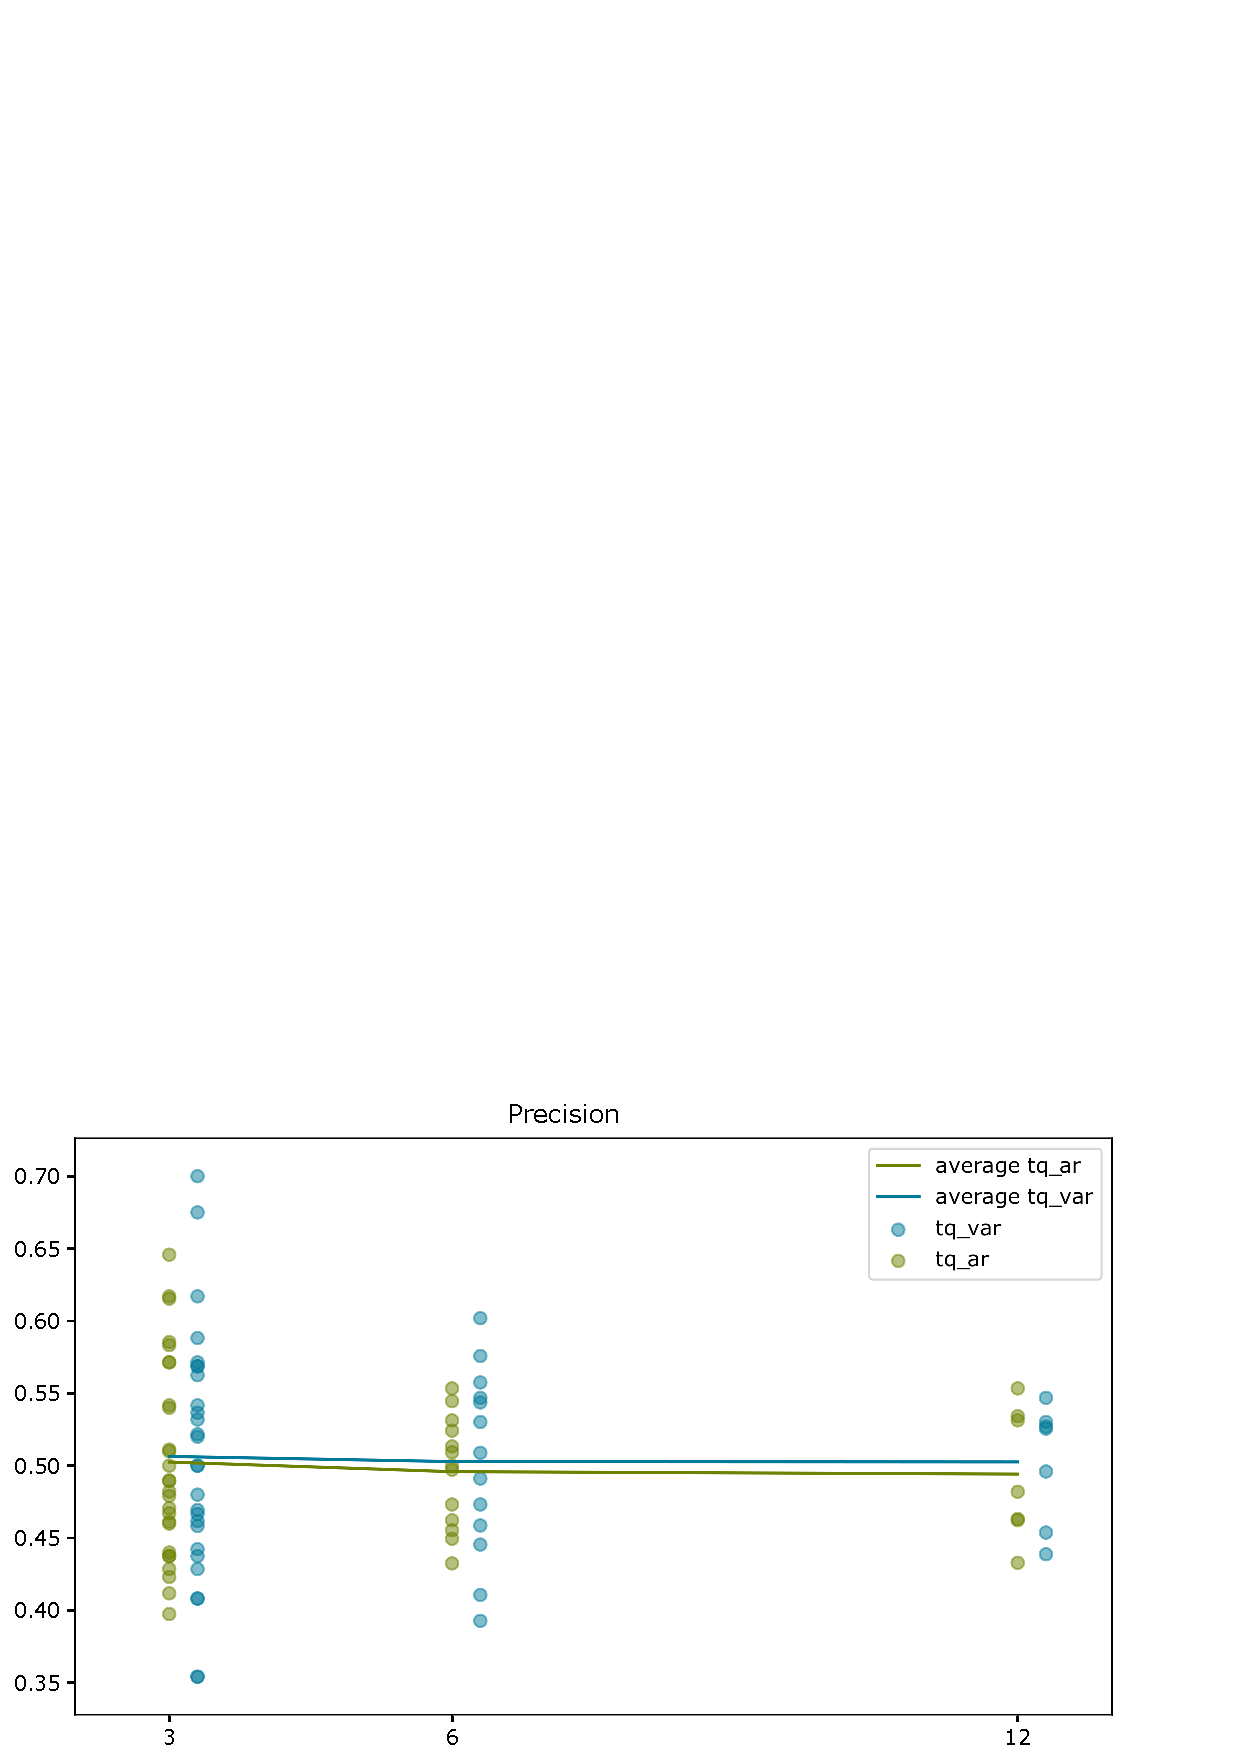
\includegraphics[width=\linewidth]{images/comparison_prec.pdf}
%		\caption[Trefferquote der beiden Modelle im Vergleich]{Präzision der beiden Modelle im Vergleich\footnotemark.}
%	\end{minipage}
%	\hspace{.1\linewidth} %Abstand dazwischen
%	\begin{minipage}[b]{.4\linewidth}
%		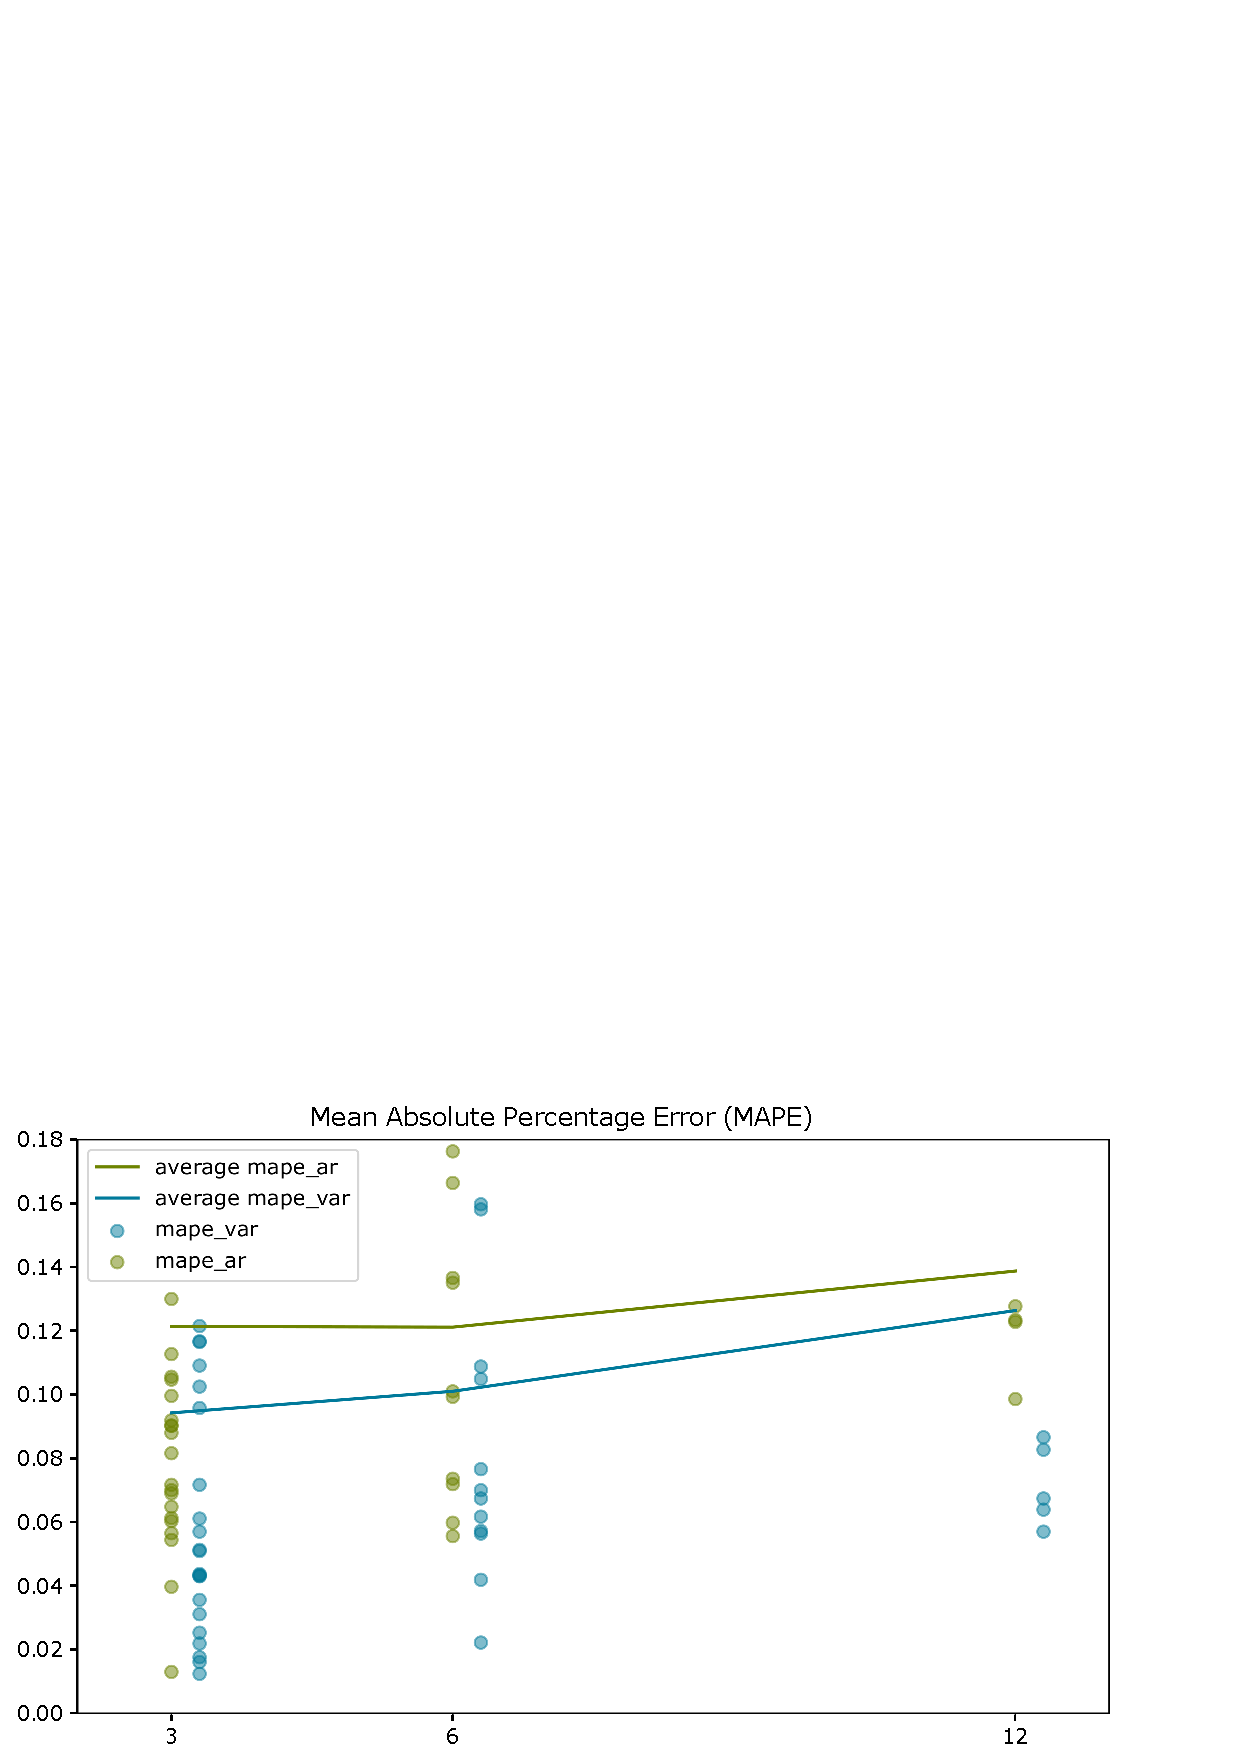
\includegraphics[width=\linewidth]{images/comparison_mape.pdf}
%		\caption[MAPE der beiden Modelle im Vergleich]{MAPE der beiden Modelle im Vergleich\footnotemark.}
%	\end{minipage}
%	\label{fig:forecast-accuracy}
%\end{figure}
%\footnotetext{Eigene Darstellung.}

\begin{figure}[H]
	\centering
	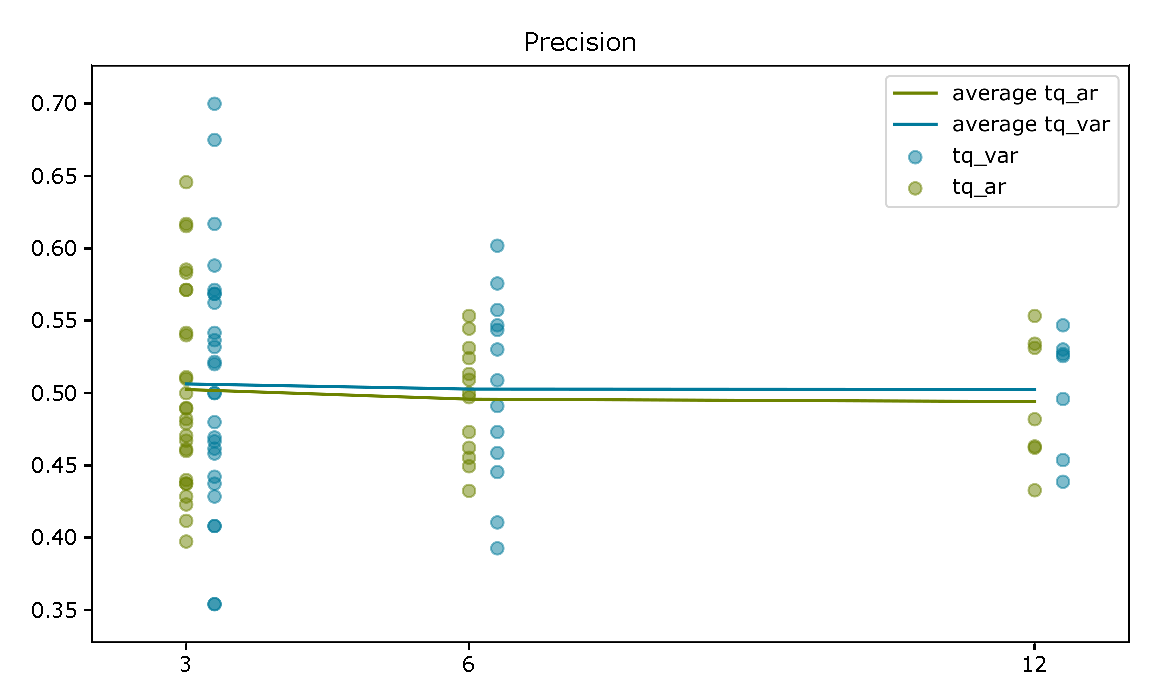
\includegraphics[width=.65\textwidth]{images/comparison_prec.eps}
	\caption[Trefferquote der beiden Modelle im Vergleich]{Präzision der beiden Modelle im Vergleich\footnotemark.}
	\label{fig:forecast-accuracy-prec}
\end{figure}
\footnotetext{Eigene Darstellung.}

\begin{figure}[H]
	\centering
	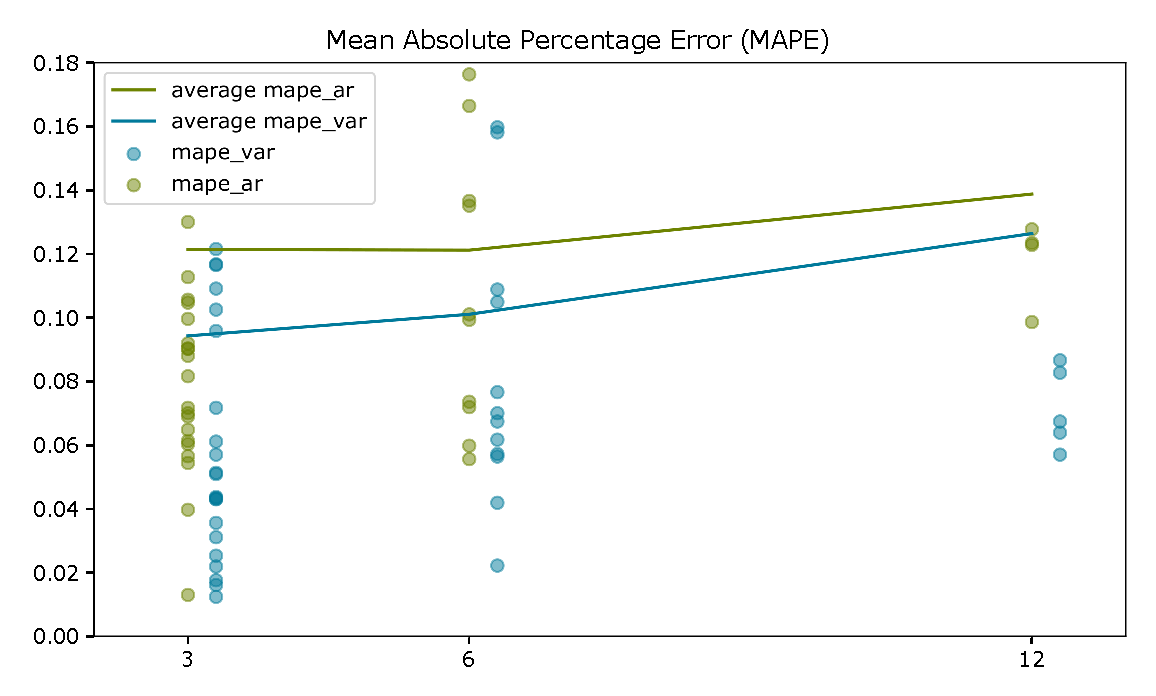
\includegraphics[width=.65\textwidth]{images/comparison_mape.eps}
	\caption[MAPE der beiden Modelle im Vergleich]{MAPE der beiden Modelle im Vergleich\footnotemark.}
	\label{fig:forecast-accuracy-mape}
\end{figure}
\footnotetext{Eigene Darstellung.}

Man erkennt anhand der Trefferquoten in Abbildung \ref{fig:forecast-accuracy-prec}, dass durch Hinzunahme der Sentiment-Variablen eine Verbesserung der Prognose möglich ist. Die Verbesserung liegt allerdings nur im Bereich von wenigen Prozentpunkten. Der MAPE in Abbildung \ref{fig:forecast-accuracy-mape} zeigt ein ähnliches Bild. Im VAR-Modell unter Einbeziehung der Sentiment-Variablen konnte der MAPE reduziert werden. Die Verbesserung der Prognose ist dabei unabhängig von der Länge des Zeitraums.\\


% ------------------------------------------------------------------------------------------------------------------------ %
%%% Kapitel 5: Kritische Betrachtung und Ausblick
% ------------------------------------------------------------------------------------------------------------------------ %
\newpage
\chapter{Kritische Betrachtung und Ausblick}
In diesem Kapitel wird eine Zusammenfassung der Ergebnisse gegeben sowie Stärken und Schwächen des Modells diskutiert. Außerdem wird ein Ausblick auf Anpassungen des Modells für eine Weiterführung gegeben.\\

Für die Erzeugung eines Textkorpus muss zunächst ein Unternehmen ausgewählt werden, dessen zugehörige Tweets analysiert werden sollen. In dieser Arbeit wurden ausschließlich "`Global Player"' ausgewählt, also Unternehmen, die weltweit agieren und deren Handeln ausreichend in den sozialen Netzwerken diskutiert wird.
Kleinere Unternehmen eignen sich aufgrund einer geringen Anzahl von Tweets nicht für die Analyse.
Die Analyse beschränkte sich außerdem nur auf Tweets in englischer Sprache, da für verschieden Sprachen verschiedene Lexika für die Sentiment-Analyse benötigt werden. Der analysierbare Textkorpus könnte dahingehend erweitert werden, indem mehrere Sprachen zur Analyse hinzugezogen werden.\\
%Die Auswahl wird dadurch weiter eingeschränkt, dass für eine Prognose des Aktienkurses ausschließlich Aktiengesellschaften ausgewählt werden können. Während in anderen Ländern (z. B. den USA) ein Großteil der großen Unternehmen die Aktiengesellschaft als Rechtsform gewählt hat, ist z. B. in Deutschland der Anteil an großen Unternehmen in anderen Rechtsformen deutlich höher.

In der Datenerhebung wurden ca. 350.000 Tweets erfasst und analysiert, von denen jedoch nur ca. $61\%$ (ca. 212.000 Tweets) erfolgreich analysiert und verwertet werden konnten. Durch den relativ großen Anteil nicht analysierbarer Tweets geht ein erheblicher Anteil an Informationen verloren. Durch eine Erweiterung der Methoden der Sentiment-Analyse, vorallem durch Verwendung umfangreicherer Lexika, könnte der Anteil der analysierbaren Tweets noch deutlich gesteigert werden. Auf maschinellem Lernen basierende Methoden der Sentiment-Analyse erzielen derzeit zwar noch schlechtere Ergebnisse bei der Genauigkeit der Analyse, erreichen jedoch meistens einen höheren Anteil analysierter Tweets\footnote{Siehe Abschnitt \ref{subsec:lexicon-based}.}. Durch die Kombination der beiden Methoden und die daraus resultierenden Synergieeffekte könnten sich bessere Ergebnisse in der Analyse erzielen lassen.\\

Für die Entwicklung einer Sentiment-Variablen wurde außerdem ausschließlich die Polarität eines Textes verwendet. Menschliche Emotionen sind jedoch wesentlich komplexer und lassen sich nicht auf einer eindimensionalen Skala abbilden. Mit dieser Reduktion ist daher auch ein Informationsverlust verbunden. Durch komplexere Sentiment-Analyse-Modelle könnten auch diese in den Texten enthaltenen Informationen analysiert und verwendet werden. Es gibt bereits Ansätze, die neben der Polarität auch die Subjektivität eines Textes ermitteln können, sowie komplexere Ansätze wie z. B. das "`Profile of Mood States"', mit dem Emotionen in sechs verschiedenen Dimensionen ausgedrückt werden. Eine Verwendung komplexere Sentiment-Analyse-Modelle könnte also ein genaueres Stimmungsbild liefern und eventuell bessere Prognosen liefern.\\

Die Ergebnisse des vorigen Kapitels zeigen, dass sich mithilfe der Daten aus sozialen Netzwerken ein Prognosemodell für Aktienkurse verbessern lässt. Dabei werden jedoch schnell die Grenzen des Modells sichtbar.
Mit nur wenigen Prozentpunkten fällt die Verbesserung des Modells durch Hinzunahme der Sentiment-Variablen allgemein sehr schwach aus.
Dennoch konnte das Modell die erwartete Genauigkeit eines "`einfachen Ratens"' von $50\%$ übertreffen.\\

Weitere Verbesserungsmöglichkeiten gibt es bei der Modellbildung.
Durch die zahlreichen Methoden zur Fehleranalyse, die das VAR-Modell ermöglicht, könnte ein besser angepasstes Modell entwickelt und damit eine präzisere Vorhersage erzeugt werden.
Dabei könnten speziell für Finanzzeitreihen entwickelte Modelle wie z. B. ARCH-Zeitreihen ebenfalls verwendet werden, um die Prognose zu verbessern. \\


% ------------------------------------------------------------------------------------------------------------------------ %
%%% Kapitel 6: Fazit
% ------------------------------------------------------------------------------------------------------------------------ %
\newpage
\chapter{Fazit}
Diese Arbeit wurde durch die Fragestellung motiviert, ob sich die Stimmung in sozialen Netzwerken auf den Aktienkurs eines Unternehmens auswirkt und ob sich mithilfe dieser Informationen eine Prognose für einen Aktienkurs ermitteln lässt. Als Einführung wurde dafür zunächst ein Überblick über Forschungsarbeiten mit ähnlichen Fragestellungen gegeben und deren Methoden verglichen. Da für eine eigene Vorhersage zunächst eine Variable benötigt wird, die die Stimmung in sozialen Netzwerken beschreibt, wurden zunächst die Grundlagen der Textverarbeitung in der Computerlinguistik dargestellt und darauf aufbauend ein Modell zur Textverarbeitung entwickelt. Anschließend wurden zu verschiedenen Unternehmen Tweets abgerufen und zu einem Textkorpus zusammengefasst. Zur Analyse der Stimmung eines Textkorpus ist eine Sentiment-Analyse notwendig. Die verschiedenen Modelle zur Ermittlung des Sentiments wurden dazu zunächst vorgestellt und schließlich die Textkorpora analysiert, woraus eine Sentiment-Variable abgeleitet werden konnte.\\

Um die Frage zu beantworten, ob ein Prognosemodell durch Hinzunahme einer Sentiment-Variablen verbessert werden kann, muss zunächst ein Referenzmodell aufgestellt werden. Hierzu wurde das Modell der Vektorautoregression vorgestellt, die Schätzung der Parameter und der Ordnung erörtert und aufgezeigt, wie sich anhand des Modells Prognosen erzeugen lassen. Mit dem Referenzmodell wurde zunächst eine Vorhersage des Aktienkurses ohne Einbeziehung der Sentiment-Variablen getroffen. Anschließend wurde dem Prognosemodell die Sentiment-Variable sowie die Anzahl täglicher Tweets hinzugefügt und die daraus resultierenden Prognosen wurden mit dem Referenzmodell verglichen. Beim Vergleich der Trefferquoten der beiden Modelle konnte gezeigt werden, dass sich durch Sentiment-Variablen eine Prognose von Aktienkursen verbessern lässt.\\

In einer kritischen Betrachtung wurden abschließend einige Schwächen aufgezeigt und es konnten Impulse für eine Fortführung der Arbeit gegeben werden.\\



% ------------------------------------------------------------------------------------------------------------------------ %
%%% Mathematischer Anhang
% ------------------------------------------------------------------------------------------------------------------------ %
\appendix
\addtocontents{toc}{\protect\setcounter{tocdepth}{0}}				% do not show chapters in toc
\chapter{Mathematischer Anhang}


%%% A.1: Definitionen -----------------------------------------------------------------------------------------------------%
\section{Definitionen}
\label{sec:definitions}

% PRÄZISION
\vspace{1.5cm}
\begin{Definition}[Präzision]
    Die \textbf{Präzision} P eines binären Klassifikators ist der Anteil der korrekt als positiv klassifizierten Ergebnisse an der Gesamtheit der als positiv klassifizierten Ergebnisse:
    \begin{equation}
        P(\text{tatsächlich \ positiv} \ | \ \text{positive \ Klassifikation}) = \frac{r_p}{r_p + f_p},
    \end{equation}
    wobei $f_p$ der Anteil der falschen positiven Klassifizierten und $r_p$ der Anteil der richtigen positiven Klassifikationen ist.\\
    
    Auch: \textit{Genauigkeit, positiver Vorhersagewert, precision}
\end{Definition}


% TREFFERQUOTE
\vspace{1.5cm}
\begin{Definition}[Trefferquote]
    Die \textbf{Trefferquote} R eines binären Klassifikators ist der Anteil der korrekt als positiv klassifizierten Ergebnisse an der Gesamtheit der tatsächlich positiven Ergebnisse:
    \begin{equation}
        P(\text{positive \ Klassifikation} \ | \ \text{tatsächlich \ positiv}) = \frac{r_p}{r_p + f_n},
    \end{equation}
    wobei $f_n$ der Anteil der falschen negativ Klassifizierten und $r_p$ der Anteil der richtigen positiven Klassifikationen ist.\\
    
    Auch: \textit{Sensitivität, Empfindlichkeit, recall, hit rate}
	\label{def:tq}
\end{Definition}


% F-MASS
\vspace{1.5cm}
\begin{Definition}[F-Maß]
    Das \textbf{$F_\alpha$-Maß} ist ein kombiniertes Maß für die Beurteilung der Güte eines binären Klassifikators. Es ist definiert durch
    \begin{equation}
        F_{\alpha} = (1 + \alpha^2) \cdot \frac{P \cdot R}{\alpha^2 \cdot P + R}
    \end{equation}
    mit der Präzision $P$ und der Trefferquote $R$.\\
    
    Das \textbf{$F_1$-Maß} (oft auch nur F-Maß genannt) ergibt sich als Spezialfall bei einer Gleichgewichtung von Präzision und Trefferquote:
    \begin{equation}
        F_1 = (1 + \alpha^2) \cdot \frac{P \cdot R}{\alpha^2 \cdot P + R} 
            = 2 \cdot \frac{P \cdot R}{P + R}
    \end{equation}
\end{Definition}



% MAPE
\vspace{1.5cm}
\begin{Definition}[Mean absolute percentage error]
    Der \textbf{mittlere absolute prozentuale Fehler} (mean absolute percentage error, MAPE) ist ein Maß für die Prognosegüte:
    \begin{equation}
        MAPE = \frac{1}{n} \sum_{i = 1}^{n} \begin{vmatrix}\frac{a_t - f_t}{a_t} \\ \end{vmatrix} \ ,
    \end{equation}
    wobei $a_t$ der tatsächliche Wert und $f_t$ der Vorhersagewert ist.
		\label{def:mape}
\end{Definition}



%%% A.2: Penn Treebank Tagset ---------------------------------------------------------------------------------------------%
\newpage
\section{POS Tagsets}
\label{app:pos-tagsets}
\begin{table}[H]
	\centering
	\begin{tabular}{ |p{1cm} p{5cm}|p{1cm} p{5cm}|  }
		\hline
		\rowcolor{tubs_blue_light}
		\multicolumn{4}{|c|}{\textbf{The Penn Treebank POS tagset\footnotemark}} \\
		\hline
		CC&Coordinating conjunction&TO&\textit{to}\\
		CD&Cardinal number&UH&Interjection\\
		DT&Determiner&VB&Verb, base form\\
		EX&Existential \textit{there}&VDB&Verb, past tense\\
		FW&Foreign Word&VBG&Verb, gerund/present participle\\
		IN&Preposition\/subordinating conjunction&VBN&Verb, past participle\\
		JJ&Adjective&VBP&Verb, non-3rd ps. sing. present\\
		JJR&Adjective, comparative&VBZ&Verb, 3rd ps. sing. present\\
		JJS&Adjective, superlative&WDT&\textit{wh}-determiner\\
		LS&List item marker&WP&\textit{wh}-pronoun\\
		MD&Modal&WP\$ &Possessive \textit{wh}-pronoun\\
		NN&Noun, singular or mass&WRB&\textit{wh}-adverb\\
		NNS&Noun, plural&\# &Pound sign\\
		NNP&Proper noun, singular&\$ &Dollar sign\\
		NNPS&Proper noun, plural&.&Sentence-final punctuation\\
		PDT&Predeterminer&,&Comma\\
		POS&Possessice ending&:&Colon, semi-colon\\
		PRP&Personal pronoun&(&Left bracket character\\
		PP\$ &Possessive pronoun&)&Right bracket character\\
		RB&Adverb&" &Straight double quote\\
		RBR&Adverb, comparative&`&Left open single quote\\
		RBS&Adverb, superlative&``&Left open double quote\\
		RP&Particle&'&Right close single quote\\
		SYM&Symbol (mathematical or scientific)&''&Right close double quote\\
		\hline
	\end{tabular}
	\caption[Abkürzungen des Penn-Treebank-Tagsets]{Abkürzungen des Penn-Treebank-Tagsets. Das Tagset beinhaltet alle Abkürzungen für die verschiedenen parts-of-speech, die im Zuge der Tokenisierung einem Satzteil zugewiesen werden können.}
	\label{tab:pos-tagsets}
\end{table}
\footnotetext{Vgl. \citet{marcus1993}, S. 317.}


%%% A.3: Vektorisierung von Matrizen -------------------------------------------------------------------------------------%
\newpage
\section{Vektorisierung von Matrizen}
\label{app:matrixvector}
Einige Sätze und Beweise verwenden die Vektorisierung von Matrizen. Dabei handelt es sich um eine lineare Abbildung, die Matrizen in einen Vektor umwandelt. Sie wird meist durch $vec(A)$ notiert. Die Abbildung wandelt eine Matrix $A \in \mathbb{R}^{m \times n}$ in einen Vektor $vec(A) \in \mathbb{R}^{mn \times 1}$ um, indem die Spalten der Matrix "`aufeinander gestapelt"' werden, also
\begin{equation*}
    vec(A) = vec\left( \begin{bmatrix}
    a_{1,1} & \cdots & a_{1,n} \\
    \vdots & \ddots & \vdots \\
    a_{m,1} & \cdots & a_{m,n} \\
    \end{bmatrix} \right)
    =
    [a_{1,1} , \ldots , a_{m,1}, a_{1,2}, \ldots , a_{m,2} , \ldots , a_{m,n}]^T
\end{equation*}

Oft wird diese Schreibweise in Zusammenhang mit dem Kronecker-Produkt verwendet, da man so Matrixmultiplikationen als Lineare Abbildung von Matrizen schreiben kann. Dabei gilt für vektorisierte Matrizen (passender Dimension):
\begin{equation*}
    vec(AB) = (I \otimes A) vec(B) = (B^T \otimes I) vec(A)
\end{equation*}
\begin{equation*}
    vec(ABC) = (I \otimes AB) vec(C) = (C^T B^T \otimes I) vec(A)
\end{equation*}

mit der Einheitsmatrix $I$\footnote{Vgl. \cite{luetkepohl2005}, S. 661 ff.}.




%%% A.4: Notationen des VAR(p)-Modells -----------------------------------------------------------------------------------%
\newpage
\section{Notationen des VAR(p)-Modells}
\label{app:var-notations}

% Matrixschreibweise
\subsection*{Matrixschreibweise}
\label{app:var-notations-matrix}
Ein VAR(p)-Modell mit $k$ Variablen für $T+1$ Beobachtungen $(y_p, ..., y_T)$ lässt sich in unterschiedlichen Notationen darstellen. In Abschnitt \ref{sec:var-estimation} wird diese kurze Matrixschreibweise verwendet\footnote{Vgl. \citet{luetkepohl2005}, S. 70.}:

\begin{Korollar}[Matrixschreibweise des VAR(p)-Modells]
    \begin{flalign*}
        Y &= B Z + U&\\
    \end{flalign*}
    
    mit
    
    \begin{flalign*}
        Y &= [y_{p} \ y_{p+1} \ \cdots \ y_{T}] = \begin{bmatrix}y_{1,p} & y_{1,p+1} & \cdots & y_{1, T} \\ y_{2,p} & y_{2,p+1} & \cdots & y_{2, T} \\ \vdots & \vdots & \vdots & \vdots \\ y_{k,p} & y_{k,p+1} & \cdots & y_{k, T}\end{bmatrix} &\\
    \end{flalign*}
    
    \begin{flalign*}
        B &= [c \ A_1 \ A_2 \ \cdots \ A_p] = \begin{bmatrix}
            c_1 & a_{1,1}^{1} & a_{1,2}^{1} & \cdots & a_{1,k}^{1} & \cdots & a_{1,1}^{p} & a_{1,2}^{p} & \cdots & a_{1,k}^{p} \\
            c_2 & a_{2,1}^{1} & a_{2,2}^{1} & \cdots & a_{2,k}^{1} & \cdots & a_{2,1}^{p} & a_{2,2}^{p} & \cdots & a_{2,k}^{p} \\
            \vdots & \vdots & \vdots & \ddots & \vdots & \cdots & \vdots & \vdots & \ddots & \vdots \\
            c_k & a_{k,1}^{1} & a_{k,2}^{1} & \cdots & a_{k,k}^{1} & \cdots & a_{k,1}^{p} & a_{k,2}^{p} & \cdots & a_{k,k}^{p} \\
        \end{bmatrix} &\\
    \end{flalign*}
    
    \begin{flalign*}
        Z &= \begin{bmatrix}
            1 & 1 & \cdots & 1 \\
            y_{p-1} & y_{p} & \cdots & y_{T-1} \\
            y_{p-2} & y_{p-1} & \cdots & y_{T-2} \\
            \vdots & \vdots & \ddots & \vdots \\
            y_{0} & y_{1} & \cdots & y_{T-p} \\
        \end{bmatrix}
        =
        \begin{bmatrix}
            1 & 1 & \cdots & 1 \\
            y_{1,p-1} & y_{1,p} & \cdots & y_{1,T-1} \\
            y_{2,p-1} & y_{2,p} & \cdots & y_{2,T-1} \\
            \vdots & \vdots & \ddots & \vdots \\
            y_{k,p-1} & y_{k,p} & \cdots & y_{k,T-1} \\
            y_{1,p-2} & y_{1,p-1} & \cdots & y_{1,T-2} \\
            y_{2,p-2} & y_{2,p-1} & \cdots & y_{2,T-2} \\
            \vdots & \vdots & \ddots & \vdots \\
            y_{k,p-2} & y_{k,p-1} & \cdots & y_{k,T-2} \\
            \vdots & \vdots & \ddots & \vdots \\
            y_{1,0} & y_{1,1} & \cdots & y_{1,T-p} \\
            y_{2,0} & y_{2,1} & \cdots & y_{2,T-p} \\
            \vdots & \vdots & \ddots & \vdots \\
            y_{k,0} & y_{k,1} & \cdots & y_{k,T-p} \\
        \end{bmatrix} &\\
    \end{flalign*}
        
    \begin{flalign*}
        U &= [e_{p} \ e_{p+1} \ \cdots \ e_{T}]
        =
        \begin{bmatrix}
            e_{1,p} & e_{1,p+1} & \cdots & e_{1,T} \\
            e_{2,p} & e_{2,p+1} & \cdots & e_{2,T} \\
            \vdots & \vdots & \ddots & \vdots \\
            e_{k,p} & e_{k,p+1} & \cdots & e_{k,T} \\
        \end{bmatrix}
        &\\
    \end{flalign*}
\end{Korollar}

\clearpage

% Rekursive Darstellung
\subsection*{Rekursive Darstellung}
\label{app:var-notations-recursive}
Ein $VAR(1)$-Prozess kann durch rekursives Einsetzen dargestellt werden als:

\begin{flalign*}
	y_1 &= \nu + A_1 y_0 + u_1 \\
	y_2 &= \nu + A_1 y_1 + u_2 = \nu + A_1 (\nu + A_1 y_0 + u_1) + u_2 \\
	    &= (I_K + A_1) \nu + A_1^2 y_0 + A_1 u_1 + u_2 \\
			&\vdots \\
	y_t &= (I_K + A_1 + \ldots + A_1^{t-1}) \nu + A_1^t y_0 + \sum_{i=0}^{t-1} A_1^i u_{t-i}
\end{flalign*}







%%% A.5: Rückführung von VAR(p) auf VAR(1) -------------------------------------------------------------------------------%
\newpage
\section{Rückführung von VAR(p) auf VAR(1)}
\label{app:varp-var1}
\begin{Korollar}[Rückführung von VAR(p) auf VAR(1)\footnotemark]
		Für höhere Ordnungen $p$ kann der Prozess $VAR(p)$ auf einen $VAR(1)$-Prozess zurückgeführt werden. Dazu sei $y_t = \nu + A_1 y_{t-1} + \ldots + A_p y_{t-p} + u_t \ , \ t=0, \ \pm 1, \ \pm2, \ \ldots$ ein $VAR(p)$-Prozess.\\
		Zu diesem $VAR(p)$-Prozess kann nun ein entsprechender $Kp$-dimensionaler $VAR(1)$"=Prozess
		\begin{flalign*}
        Y_t &= \nu + A Y_{t-1} + U_t &
    \end{flalign*}
	definiert werden, indem
	\begin{flalign*}
		Y_t &:= \begin{bmatrix}y_t \\ y_{t-1} \\ \vdots \\ y_{t-p+1} \\ \end{bmatrix} \ , \ \nu := \begin{bmatrix} \nu \\ 0 \\ \vdots \\ 0 \end{bmatrix} \ , \\
		A &:= \begin{bmatrix} A_1 & A_2 & \cdots & A_{p-1} & A_p \\
													I_K & 0 & \cdots & 0 & 0 \\
													0 & I_K & \ & 0 & 0 \\
													\vdots & \ & \ddots & \vdots & \vdots \\
													0 & 0 & \cdots & I_K & 0 \\\end{bmatrix} \ , \
				  \begin{bmatrix}u_t \\ 0 \\ \vdots \\ 0 \end{bmatrix}
	\end{flalign*}
	gewählt werden.\\
\end{Korollar}
\footnotetext{Vgl. \cite{luetkepohl2005}, S. 15 f.}



% ------------------------------------------------------------------------------------------------------------------------ %
%%% Quellcode-Anhang
% ------------------------------------------------------------------------------------------------------------------------ %
\chapter{Quellcode-Anhang}
%\lstlistoflistings								% List of listings

%%% B.1: SQL -------------------------------------------------------------------------------------------------------------%
\section{SQL}
Die in dieser Arbeit verwendete Datenbank arbeitet mit dem gemeinfreien, relationalen Datenbanksystem SQLite. SQLite unterstützt den SQL-92-Standard. Alle Abfragen auf der SQLite-Datenbank werden demnach mit der Structured Query Language \textbf{SQL} durchgeführt.\\


\begin{table}[H]
	\centering
	\begin{tabular}{| p{1cm} | p{6cm} | p{9cm} |}
		\hline
		\rowcolor{tubs_blue_light}
		Quellcode Nr. & Funktion & Beschreibung \\ \hline
		\ref{lst:sql-create-table-tweets}  &  CREATE\_TABLE\_TWEETS.sql & Erstellen der Datenbank-Tabelle 'tweets' \\ \hline
		\ref{lst:sql-create-table-searches}  &  CREATE\_TABLE\_SEARCHES.sql & Erstellen der Datenbank-Tabelle 'searches' \\ \hline
		\ref{lst:sql-create-table-stocks}  &  CREATE\_TABLE\_STOCKS.sql & Erstellen der Datenbank-Tabelle 'stocks' \\ \hline
		\ref{lst:sql-sp-remove-duplicates}  &  CREATE\_TABLE\_TWEETS.sql & Prozedur zum Entfernen von Duplikaten in der Datenbank. \\ \hline
		\ref{lst:sql-get-full-timeseries}  &  GET\_FULL\_TIME\_SERIES.sql & Prozedur zum Aggregieren der Daten und zum Erzeugen der Zeitreihe. \\ \hline
	\end{tabular}
	\caption{Übersicht der SQL-Queries}
	\label{tab:sql-queries}
\end{table}



%%% B.1.1: Datenbank erstellen -------------------------------------------------------------------------------------------%
\newpage
\subsection*{Erstellen der Datenbank-Tabellen}
\label{subsec:create-tables}
Die folgenden Funktionen werden verwendet, um die Datenbank-Tabellen zu erstellen.\\


% CREATE TABLE 'tweets'
\begin{tabular}{| >{\columncolor{tubs_blue_light}} p{3cm} | p{12cm} |}
    \hline
    \textbf{Funktion} & CREATE\_TABLE\_TWEETS.sql \\ \hline
    \textbf{Beschreibung} & Erzeugt die Tabelle 'tweets' zum Speichern der abgerufenen Tweets. \\ \hline
    \textbf{Aufruf} & Der Aufruf kann mittels Python (package \textit{sqlite3}) oder mit einem Datenbankmanagementsystem (z. B. SQLiteStudio) erfolgen. \\  \hline
\end{tabular}\\

\lstinputlisting[language = SQL,
                 label = {lst:sql-create-table-tweets},
                 caption = {SQL: Erstellen der Tabelle 'tweets'},
                 ]
                 {code/SQL_CREATE_TABLE_TWEETS.sql}

% CREATE TABLE 'tweets'
\vspace{1.5cm}
\begin{tabular}{| >{\columncolor{tubs_blue_light}} p{3cm} | p{12cm} |}
    \hline
    \textbf{Funktion} & CREATE\_TABLE\_SEARCHES.sql \\ \hline
    \textbf{Beschreibung} & Erzeugt die Tabelle 'searches', in der Informationen zu einer Suchabfrage gespeichert werden. Die Tabelle dient der Verknüpfung der Tweets aus der Tabelle 'tweets' mit den Aktienkursen aus der Tabelle 'stocks'. \\ \hline
    \textbf{Aufruf} & Der Aufruf kann mittels Python (package \textit{sqlite3}) oder mit einem Datenbankmanagementsystem (z. B. SQLiteStudio) erfolgen. \\  \hline
\end{tabular}\\
\lstinputlisting[language = SQL,
                 label = {lst:sql-create-table-searches},
                 caption = {SQL: Erstellen der Tabelle 'searches'},
                 ]
                 {code/SQL_CREATE_TABLE_SEARCHES.sql}
                 
% CREATE TABLE 'tweets'
\vspace{1.5cm}
\begin{tabular}{| >{\columncolor{tubs_blue_light}} p{3cm} | p{12cm} |}
    \hline
    \textbf{Funktion} & CREATE\_TABLE\_STOCKS.sql \\ \hline
    \textbf{Beschreibung} & Erezugt die Tabelle 'stocks' zum Speichern der Aktienkurse, die für die Prognose benötigt werden. Gespeichert werden alle Preisinformationen: high (höchster Kurs des Tages), low (niedrigster Kurs des Tages), open (Eröffnungskurs), close (Schlusskurs), adj\_close (angepasster Schlusskurs, der Kapitalmaßnahmen und Ausschüttungen berücksichtigt), volume (Handelsvolumen). \\ \hline
    \textbf{Aufruf} & Der Aufruf kann mittels Python (package \textit{sqlite3}) oder mit einem Datenbankmanagementsystem (z. B. SQLiteStudio) erfolgen. \\  \hline
\end{tabular}\\
\lstinputlisting[language = SQL,
                 label = {lst:sql-create-table-stocks},
                 caption = {SQL: Erstellen der Tabelle 'stocks'},
                 ]
                 {code/SQL_CREATE_TABLE_STOCKS.sql}


%%% B.1.2: Stored Procedures ---------------------------------------------------------------------------------------------%
\subsection*{Stored Procedures}

% SP_REMOVE_DUPLICATES
\begin{tabular}{| >{\columncolor{tubs_blue_light}} p{3cm} | p{12cm} |}
    \hline
    \textbf{Funktion} & SP\_REMOVE\_DUPLICATES.sql \\ \hline
    \textbf{Beschreibung} & Entfernt doppelt vorhandene Datensätze (Duplikate) aus der Datenbank. \\ \hline
    \textbf{Aufruf} & Der Aufruf kann mittels Python (package \textit{sqlite3}) oder mit einem Datenbankmanagementsystem (z. B. SQLiteStudio) erfolgen. \\  \hline
\end{tabular}\\
\lstinputlisting[language = SQL,
                 label = {lst:sql-sp-remove-duplicates},
                 caption = {SQL: Entfernen von Duplikaten},
                 ]
                 {code/SQL_SP_REMOVE_DUPLICATES.sql}


% SP_FLAG_FAULTY
\vspace{1.5cm}
\begin{tabular}{| >{\columncolor{tubs_blue_light}} p{3cm} | p{12cm} |}
    \hline
    \textbf{Funktion} & SP\_FLAG\_FAULTY.sql \\ \hline
    \textbf{Beschreibung} & Entfernt fehlerhafte Datensätze aus der Datenbank. Hier wurde lediglich die Länge des Tweets als Indikator für einen Fehler verwendet. Die Kriterien zur Identifikation können aber beliebig erweitert werden. \\ \hline
    \textbf{Aufruf} & Der Aufruf kann mittels Python (package \textit{sqlite3}) oder mit einem Datenbankmanagementsystem (z. B. SQLiteStudio) erfolgen. \\  \hline
\end{tabular}\\
\lstinputlisting[language = SQL,
                 label = {lst:sql-sp-flag-faulty},
                 caption = {SQL: Identifizieren fehlerhafter Datensätze},
                 ]
                 {code/SQL_SP_FLAG_FAULTY.sql}


%%% B.1.3: Zeitreihe erzeugen --------------------------------------------------------------------------------------------%
\subsection*{Erzeugen der Zeitreihen}

% GET_FULL_TIMESERIES
\begin{tabular}{| >{\columncolor{tubs_blue_light}} p{3cm} | p{12cm} |}
    \hline
    \textbf{Funktion} & SP\_GET\_FULL\_TIMESERIES.sql \\ \hline
    \textbf{Beschreibung} & Aggregiert die Daten (Tweets und Kursdaten) zu einem Datensatz für die Regressionsanalyse. \\ \hline
    \textbf{Aufruf} & Der Aufruf kann mittels Python (package \textit{sqlite3}) oder mit einem Datenbankmanagementsystem (z. B. SQLiteStudio) erfolgen. \\  \hline
\end{tabular}\\
\lstinputlisting[language = SQL,
                 label = {lst:sql-get-full-timeseries},
                 caption = {SQL: Erzeugen der Zeitreihen für die Regressionsanalyse},
                 ]
                 {code/SQL_GET_FULL_TIMESERIES.sql}



%%% B.2: Python -----------------------------------------------------------------------------------------------------------%
\newpage
\section{Python}
Die Implementierung erfolgte in Python 3.6.4. Die meisten Funktionen sind mit Python 3.7 kompatibel, ein ausführlicher Test aller Funktionen wurde für andere Versionen jedoch nicht durchgeführt. Mit Python 2 und Python 3.8 kommt es zu Kompatibilitätsproblemen.\\

\begin{table}[H]
	\centering
	\begin{tabular}{| p{2cm} | p{1cm} | p{4cm} | p{7.5cm} |}
		\hline
		\rowcolor{tubs_blue_light}
		Modul & Quellcode Nr. & Funktion & Beschreibung \\ \hline
		\textbf{database} & \ref{lst:python-vader-sql-batch} & add\_sentiments & Steuerung der Sentiment-Analyse \\ \hline
		\textbf{sentiment} & \ref{lst:python-get-sentiment} & get\_sentiment & Aufruf der verschiedenen Sentiment-Analyse-Modelle \\ \hline
		\ & \ref{lst:python-vader-sentiment} & vader\_sentiment & Für das VADER-Paket angepasster Funktionsaufruf zur Sentiment-Analyse \\ \hline
		\textbf{figures} & \ref{lst:python-dataset-statistics}  &  get\_dataset\_statistics & Visualisierung und Datensatz-Statistiken \\ \hline
		\textbf{regression} & \ref{lst:python-preproc-dataset}  &  preproc\_dataset & Datenaufbereitung \\ \hline
		\ & \ref{lst:python-adfuller-test}  &  adfuller\_test & Augmented Dickey-Fuller Test \\ \hline
		\ & \ref{lst:python-get-lag-order} & get\_lag\_order & Anwendung der Informationskriterien zum Ermitteln der Lag-Ordnung \\ \hline
		\ & \ref{lst:python-var-prediction} & var\_prediction & Vorhersage mit einem VAR-Modell \\ \hline
		\ & \ref{lst:python-ar-prediction} & ar\_prediction & Vorhersage mit einem AR-Modell \\ \hline
		\ & \ref{lst:python-forecast-accuracy} & forecast\_accuracy & Ermitteln der Prognosegüte \\ \hline
	\end{tabular}
	\caption{Übersicht der Python-Funktionen}
	\label{tab:python-functions}
\end{table}



%%% B.2.x Visualisierung und Datensatz-Statistiken--------------------------------------------------------------------------%
\newpage
\subsection*{Sentiment-Analyse}
\begin{tabular}{| >{\columncolor{tubs_blue_light}} p{3cm} | p{12cm} |}
    \hline
    \textbf{Funktion} & add\_sentiments\\ \hline
    \textbf{Beschreibung} & Die Funktion fragt Tweets aus der Datenbank ab, ermittelt ein Sentiment für den Text des Tweets und gibt den analysierten Tweet inklusive seiner Sentiment-Werte an die Datenbank zurück. Die Funktion dient als Wrapper für die Funktion \textit{get\_sentiment}, mit der die Sentiment-Analyse durchgeführt wird. \\ \hline
    \textbf{Aufruf} & Beim Aufruf können einige optionale Einstellungen vorgenommen werden, z. B. kann eine maximale Anzahl zu analysierender Tweets festgelegt werden. \\  \hline
\end{tabular}\\
\lstinputlisting[language = python,
                 label = {lst:python-vader-sql-batch},
                 caption = {Python: Abruf der Tweets aus der Datenbank und Aufruf der Sentiment-Analyse},
                 ]
                 {code/add_sentiments.py}

% get-sentiment
\vspace{1.5cm}
\begin{tabular}{| >{\columncolor{tubs_blue_light}} p{3cm} | p{12cm} |}
    \hline
    \textbf{Funktion} & get\_sentiments\\ \hline
    \textbf{Beschreibung} & Die Funktion steuert den Aufruf der einzelnen Sentiment-Analyse-Funktionen. \\ \hline
    \textbf{Aufruf} & Beim Aufruf kann das zu verwendende Sentiment-Analyse-Modell optional gewählt werden. Standarmäßig wird das VADER-Paket verwendet. \\  \hline
\end{tabular}\\
\lstinputlisting[language = python,
                 label = {lst:python-get-sentiment},
                 caption = {Python: Wrapper für die Funktionen zur Sentiment-Analyse},
                 ]
                 {code/get_sentiment.py}


% vader-sentiment
\vspace{1.5cm}
\begin{tabular}{| >{\columncolor{tubs_blue_light}} p{3cm} | p{12cm} |}
    \hline
    \textbf{Funktion} & vader\_sentiment\\ \hline
    \textbf{Beschreibung} & Mit der Funktion wird ein Sentiment unter Verwendung des VADER-Paketes erzeugt und zurückgegeben. \\ \hline
    \textbf{Aufruf} & Der Aufruf kann mit optionalen Argumenten erfolgen, wenn andere Rückgabe-Formate gewünscht sind. \\  \hline
\end{tabular}\\
\lstinputlisting[language = python,
                 label = {lst:python-vader-sentiment},
                 caption = {Python: Ermittlung eines Sentiments mit dem VADER-Paket.},
                 ]
                 {code/vader_sentiment.py}
								


%%% B.2.x Visualisierung und Datensatz-Statistiken--------------------------------------------------------------------------%
\newpage
\subsection*{Visualisierung und Datensatz-Statistiken}
\begin{tabular}{| >{\columncolor{tubs_blue_light}} p{3cm} | p{12cm} |}
    \hline
    \textbf{Funktion} & get\_dataset\_statistics \\ \hline
    \textbf{Beschreibung} & Funktion zum Erzeugen einer Visualisierung eines Sentiment-Datensatzes bestehend aus durchschnittlichem Sentiment, Tweet-Anzahl und Aktienkurs. \\ \hline
    \textbf{Aufruf} & Beim Aufruf können die Parameter des Datensatzes (Beginn, Ende, Name des Datensatzes) und das Ausgabeformat (statistische Werte, Graph) gewählt werden. \\  \hline
\end{tabular}\\
\lstinputlisting[language = python,
                 label = {lst:python-dataset-statistics},
                 caption = {Python: Visualisierung und Berechnung statistische Werte eines Datensatzes},
                 ]
                 {code/get_dataset_statistics.py}


%%% B.2.x Datenaufbereitung ------------------------------------------------------------------------------------------------%
\newpage
\subsection*{Datenaufbereitung}
\begin{tabular}{| >{\columncolor{tubs_blue_light}} p{3cm} | p{12cm} |}
    \hline
    \textbf{Funktion} & preproc\_dataset \\ \hline
    \textbf{Beschreibung} & Die Funktion beinhaltet alle Funktionen zur Datenaufbereitung vor der Regressionanalyse. Beim Aufruf können einige Optionen zur Datenaufbereitung angepasst werden. \\ \hline
    \textbf{Aufruf} & Beim Aufruf können einige Optionen zur Datenaufbereitung angepasst werden. Die möglichen Parameter sind im Quellcode erklärt. \\  \hline
\end{tabular}\\
\lstinputlisting[language = python,
                 label = {lst:python-preproc-dataset},
                 caption = {Python: Aufbereitung eines Datensatzes für die Analyse},
                 ]
                 {code/preproc_dataset.py}




%%% B.2.x ADF-Test --------------------------------------------------------------------------------------------------------%
\newpage
\subsection*{Augmented Dickey-Fuller Test}
\begin{tabular}{| >{\columncolor{tubs_blue_light}} p{3cm} | p{12cm} |}
    \hline
    \textbf{Funktion} & adfuller\_test \\ \hline
    \textbf{Beschreibung} & Funktion zum Ausführen des Augmented Dickey-Fuller Tests für Stationarität. Die Funktion verwendet das Paket \textit{statsmodels} und die darin implementierte Teststatistik. In der Regressionsanalyse wird die Funktion verwendet, um die Zeitreihen auf Stationarität zu prüfen. \\ \hline
    \textbf{Aufruf} & Die Funktion benötigt eine Zeitreihe in Form eines pandas DataFrame und gibt einen Wahrheitswert zurück, ob die Nullhypothese verworfen werden kann. Als optionale Parameter können z. B. Signifikanzniveau (\textit{signif}) und eine Ausgabe der Testergebnisse (\textit{print\_output = None | 'short' | 'long'}) übergeben werden. \\  \hline
\end{tabular}\\
\lstinputlisting[language = python,
                 label = {lst:python-adfuller-test},
                 caption = {Python: Implementierung des Augmented Dickey-Fuller Tests},
                 ]
                 {code/adfuller_test.py}



%%% B.2.x Informationskriterien -------------------------------------------------------------------------------------------%
\newpage
\subsection*{Informationskriterium zum Ermitteln der Ordnung}
\begin{tabular}{| >{\columncolor{tubs_blue_light}} p{3cm} | p{12cm} |}
    \hline
    \textbf{Funktion} & get\_lag\_order \\ \hline
    \textbf{Beschreibung} & Funktion zum Ermitteln der optimalen Lag-Ordnung für das VAR/AR-Modell.\\ \hline
    \textbf{Aufruf} & Die Funktion benötigt eine Zeitreihe in Form eines pandas DataFrame und gibt die optimale Lag-Ordnung zurück. Beim Funktionsaufruf können einige Parameter angepasst werden. So kann neben dem AIC auch ein anderes Informationskriterium verwendet werden. \\  \hline
\end{tabular}\\
\lstinputlisting[language = python,
                 label = {lst:python-get-lag-order},
                 caption = {Python: Ermitteln der Lag-Ordnung},
                 ]
                 {code/get_lag_order.py}


						
%%% B.2.x ar_prediction ---------------------------------------------------------------------------------------------------%
\newpage
\subsection*{Vorhersage mit einem $VAR(p)$-Modell}
\begin{tabular}{| >{\columncolor{tubs_blue_light}} p{3cm} | p{12cm} |}
    \hline
    \textbf{Funktion} & var\_prediction \\ \hline
    \textbf{Beschreibung} & Funktion zum Berechnen einer Vorhersage mit einem $VAR(p)$-Modell.\\ \hline
    \textbf{Aufruf} & Die Funktion benötigt Zeitreihen in Form eines pandas DataFrame und erweitert den DataFrame um die Vorhersagewerte, basiernd auf den Modellparametern, die an die Funktion übergeben werden können. \\  \hline
\end{tabular}\\
\lstinputlisting[language = python,
                 label = {lst:python-var-prediction},
                 caption = {Python: Vorhersage mit einem VAR(p)-Modell},
                 ]
                 {code/var_prediction.py}
						


%%% B.2.x ar_prediction ---------------------------------------------------------------------------------------------------%
\newpage
\subsection*{Vorhersage mit einem $AR(p)$-Modell}
\begin{tabular}{| >{\columncolor{tubs_blue_light}} p{3cm} | p{12cm} |}
    \hline
    \textbf{Funktion} & ar\_prediction \\ \hline
    \textbf{Beschreibung} & Funktion zum Berechnen einer Vorhersage mit einem $AR(p)$-Modell. Die Funktion wird benötigt, da die $VAR$-Klasse des Pakets \textit{statsmodels} keine Vektorautoregression mit nur einer Variablen (d.h. eine normale Autoregression) unterstützt. \\ \hline
    \textbf{Aufruf} & Die Funktion benötigt Zeitreihen in Form eines pandas DataFrame und erweitert den DataFrame um die Vorhersagewerte basierend auf den Modellparametern, die an die Funktion übergeben werden können. \\  \hline
\end{tabular}\\
\lstinputlisting[language = python,
                 label = {lst:python-ar-prediction},
                 caption = {Python: Vorhersage mit einem AR(p)-Modell},
                 ]
                 {code/ar_prediction.py}



%%% B.2.x forecast_accuracy -----------------------------------------------------------------------------------------------%
\newpage
\subsection*{Beurteilung der Prognosegüte}
\begin{tabular}{| >{\columncolor{tubs_blue_light}} p{3cm} | p{12cm} |}
    \hline
    \textbf{Funktion} & forecast\_accuracy \\ \hline
    \textbf{Beschreibung} & Berechnet einige Maße zur Beurteilung der Prognosegüte: MAPE (mean absolute percentage error), ME (mean error), MAE (mean absolute error), MPE (mean percentage error), RMSE (root-mean-square error), CORR (correlation coefficient), MINMAX, ACC\_BIN (binary accuracy = Anzahl Vorhersagen mit richtiger Richtung). Nicht alle Maße wurden für die Fehleranalyse verwendet. \\ \hline
    \textbf{Aufruf} & Die Funktion benötigt zwei Zeitreihen (Prognosewerte und echte Werte) in Form von pandas Series und gibt ein Dictionary mit den ermittelten Werten zurück. \\  \hline
\end{tabular}\\
\lstinputlisting[language = python,
                 label = {lst:python-forecast-accuracy},
                 caption = {Python: Berechnung der Prognosegüte},
                 ]
                 {code/forecast_accuracy.py}


% ------------------------------------------------------------------------------------------------------------------------ %
%%% Literaturverzeichnis
% ------------------------------------------------------------------------------------------------------------------------ %
\newpage
\printbibliography





% ------------------------------------------------------------------------------------------------------------------------ %
%%% Ende
% ------------------------------------------------------------------------------------------------------------------------ %

\end{document}